\chapter{Design and Implementation}
\label{cha:design}

This chapter presents the design and implementation of the system, focusing on the integration of the various components and the overall architecture. The system is designed to be modular, scalable, and extensible, enabling the integration of additional components as needed.

\section{Assumptions}

In this work, workload has been modeled as \textbf{Virtual Machines (VMs)}, representing the primary use case considered during the system's initial design phase. 
[WHY THIS CHOICE?]

A key limitation of this approach is that only resources supported by the cloud provider’s Kubernetes operator can be provisioned. Not all cloud resources available in a provider’s portfolio are guaranteed to have corresponding Kubernetes Custom Resources (CRs). This introduces certain constraints:


\begin{itemize}[itemsep=0.2pt, topsep=1pt]
  \item[$\bullet$] Limited resource availability: if a specific resource type (e.g., a GPU-accelerated instance or a managed database service) is not supported by the operator, it cannot be provisioned using the current system.
  \item[$\bullet$] Dependence on Operator updates: cloud providers may extend or modify the set of resources supported by their Kubernetes operators over time.
  \item[$\bullet$] Vendor-specific implementations: different cloud providers expose varying levels of support for Kubernetes-native resource provisioning, leading to potential inconsistencies across multi-cloud environments.
\end{itemize}

Despite these constraints, the system architecture remains highly adaptable, and future enhancements could incorporate alternative provisioning mechanisms. 
An example of an alternative implementation could be the direct API interactions with cloud providers to bypass operator limitations.

[TEST]

\newpage
\section{System Architecture}
\label{sec:system_architecture}

The following table provides an overview of the main components of the system and their respective functions.

\begin{table}[H]
  \centering
  \renewcommand{\arraystretch}{1.3} % Adjust row height for readability
  \begin{tabularx}{\textwidth}{| l | X |} % 'X' makes the second column auto-wrap
    \hline
    \textbf{Component} & \textbf{Function} \\
    \hline
    Krateo PlatformOps & Provides an abstraction layer for infrastructure orchestration, enabling declarative resource management and integration with cloud providers. \\
    \hline
    Cloud Providers Kubernetes Operators & Manages the provisioning and reconciliation of cloud resources within Kubernetes, ensuring the actual state matches the desired state. \\
    \hline
    Kubernetes Mutating Webhook & Intercepts and modifies API requests before they are persisted, allowing dynamic configuration adjustments with policy enforcement. \\
    \hline
    OPA Server & Evaluates authorization and policy decisions based on defined constraints and input data from Kubernetes API requests through the webhook. \\
    \hline
    OPA Policies and Data & Define the rules and contextual information used by OPA to make policy decisions, namely scheduling information \\
    \hline
    GreenOps Scheduler & Determines the optimal scheduling region and scheduling time for VMs, acting as an external data source for OPA policies. \\
    \hline
    MLflow & Allows the tracking, logging, versioning and storing of machine learning experiments for reproducibility and model lifecycle management. \\
    \hline
    KServe & Provides scalable and Kubernetes-native model serving capabilities, enabling deployment of machine learning models for inference. \\
    \hline
  \end{tabularx}
  \caption{Main components of the system and their respective functions.}
  \label{tab:system_components}
\end{table}



All the components listed in the above table are deployed inside a Kubernetes cluster. The only exception are the OPA Policies and Data which lies outside the cluster as described in section XYZ.


Differences wrt other systems described in the background section
production-ready system





\section{Krateo PlatformOps integration}

\subsection{Helm}
what is an helm chart


\subsection{Krateo}
what is krateo
developer platform


Self-service platform for multi-cloud native resources



(generic VM mapped thanks to Krateo components, what is the added value)




generic workload resource definition


how to define it

Why K8s synchronization operator from scratch was not ideal wrt using helm charts with krateo

Helm template engine (how to map to cloud provider specific resources, why is better)







\section{Multi-Cloud Integration through Kubernetes Operators}

The integration of operators from different cloud providers has enabled the development of an effective \textbf{multi-cloud system}, allowing seamless orchestration and provisioning of cloud resources across various cloud platforms. Namely, the system leverages Kubernetes operators from \textbf{Microsoft Azure}, \textbf{Google Cloud Platform (GCP)}, and \textbf{Amazon Web Services (AWS)}.

\subsection{Role of Kubernetes Operators}

Kubernetes operators work on the principle of Continuous Reconciliation, ensuring, in this case, that the desired state of the system, as defined by users, aligns with the actual state of provisioned cloud resources. In particular, Operators act as controllers that monitor, adjust, and manage external cloud resources within a Kubernetes-native environment.
Key characteristics of operators include:
\begin{itemize}[itemsep=0.2pt, topsep=1pt]
  \item[$\bullet$] Managing external cloud resources within a Kubernetes cluster, providing a \textbf{unified interface} for multi-cloud deployments.
  \item[$\bullet$] Maintaining a \textbf{real-time representation} of provisioned cloud resources within Kubernetes.
  \item[$\bullet$] Using Custom Resources (CRs) to define cloud-specific resources in a \textbf{declarative} manner.
\end{itemize}

\subsection{Strategic Shift: From Custom Operator to Krateo Core Provider}

In our approach, we opted to replace a custom Kubernetes operator (``Synchronization Operator''), originally designed to handle the \textbf{mapping} from generic to cloud-specific resources, with \textbf{Krateo Core Provider}. This decision was motivated by the need for greater flexibility and maintainability in defining multi-cloud infrastructure components. As a matter of fact, the custom operator was originally designed to handle only virtual machines (VMs) mappings and extensions to support additional cloud resources would have required significant code changes and maintenance overhead for each additional resource type added.

Therefore instead of embedding business logic directly within a custom Kubernetes operator, in the current system implementation, we leverage the capabilities of \textbf{Helm templating} to dynamically generate cloud-provider-specific resources. More precisely, another Krateo component, the \textbf{Krateo composition-dynamic-controller} is leveraging Helm templating under the hood to generate Kubernetes resources starting from helm templates.
This approach, further described in the following sections, offers several advantages:

Simplified resource management:  Helm enables a standardized way define resources without maintaining complex operator logic.
Greater extensibility:  By externalizing the logic from the operator, future modifications and integrations with additional cloud providers become easier.
Reduced maintenance overhead: Operators typically require constant updates and refinements, while Helm-based resource generation minimizes the need for frequent code changes.

It must be noted that different cloud provider adopts different design choices for their Kubernetes operators and more in general for their overall infrastructure management. Therefore, for the creation of logically similar resources, like a virtual machine, the structure and the field of the resources can be different. 
These resources typically include:
\begin{itemize}[itemsep=0.2pt, topsep=1pt]
  \item[$\bullet$] Compute resources (e.g., VM instances, virtual machine templates)
  \item[$\bullet$] Networking components (e.g., virtual networks, subnets, security groups)
  \item[$\bullet$] Storage allocations (e.g., persistent volumes, cloud disks)
  \item[$\bullet$] Access management (e.g., resource groups, roles, authentication credentials)
\end{itemize}


For the purpose of this work we defined baseline infrastructure, 

vendor lock-in.



\begin{figure}[htb]
\centering
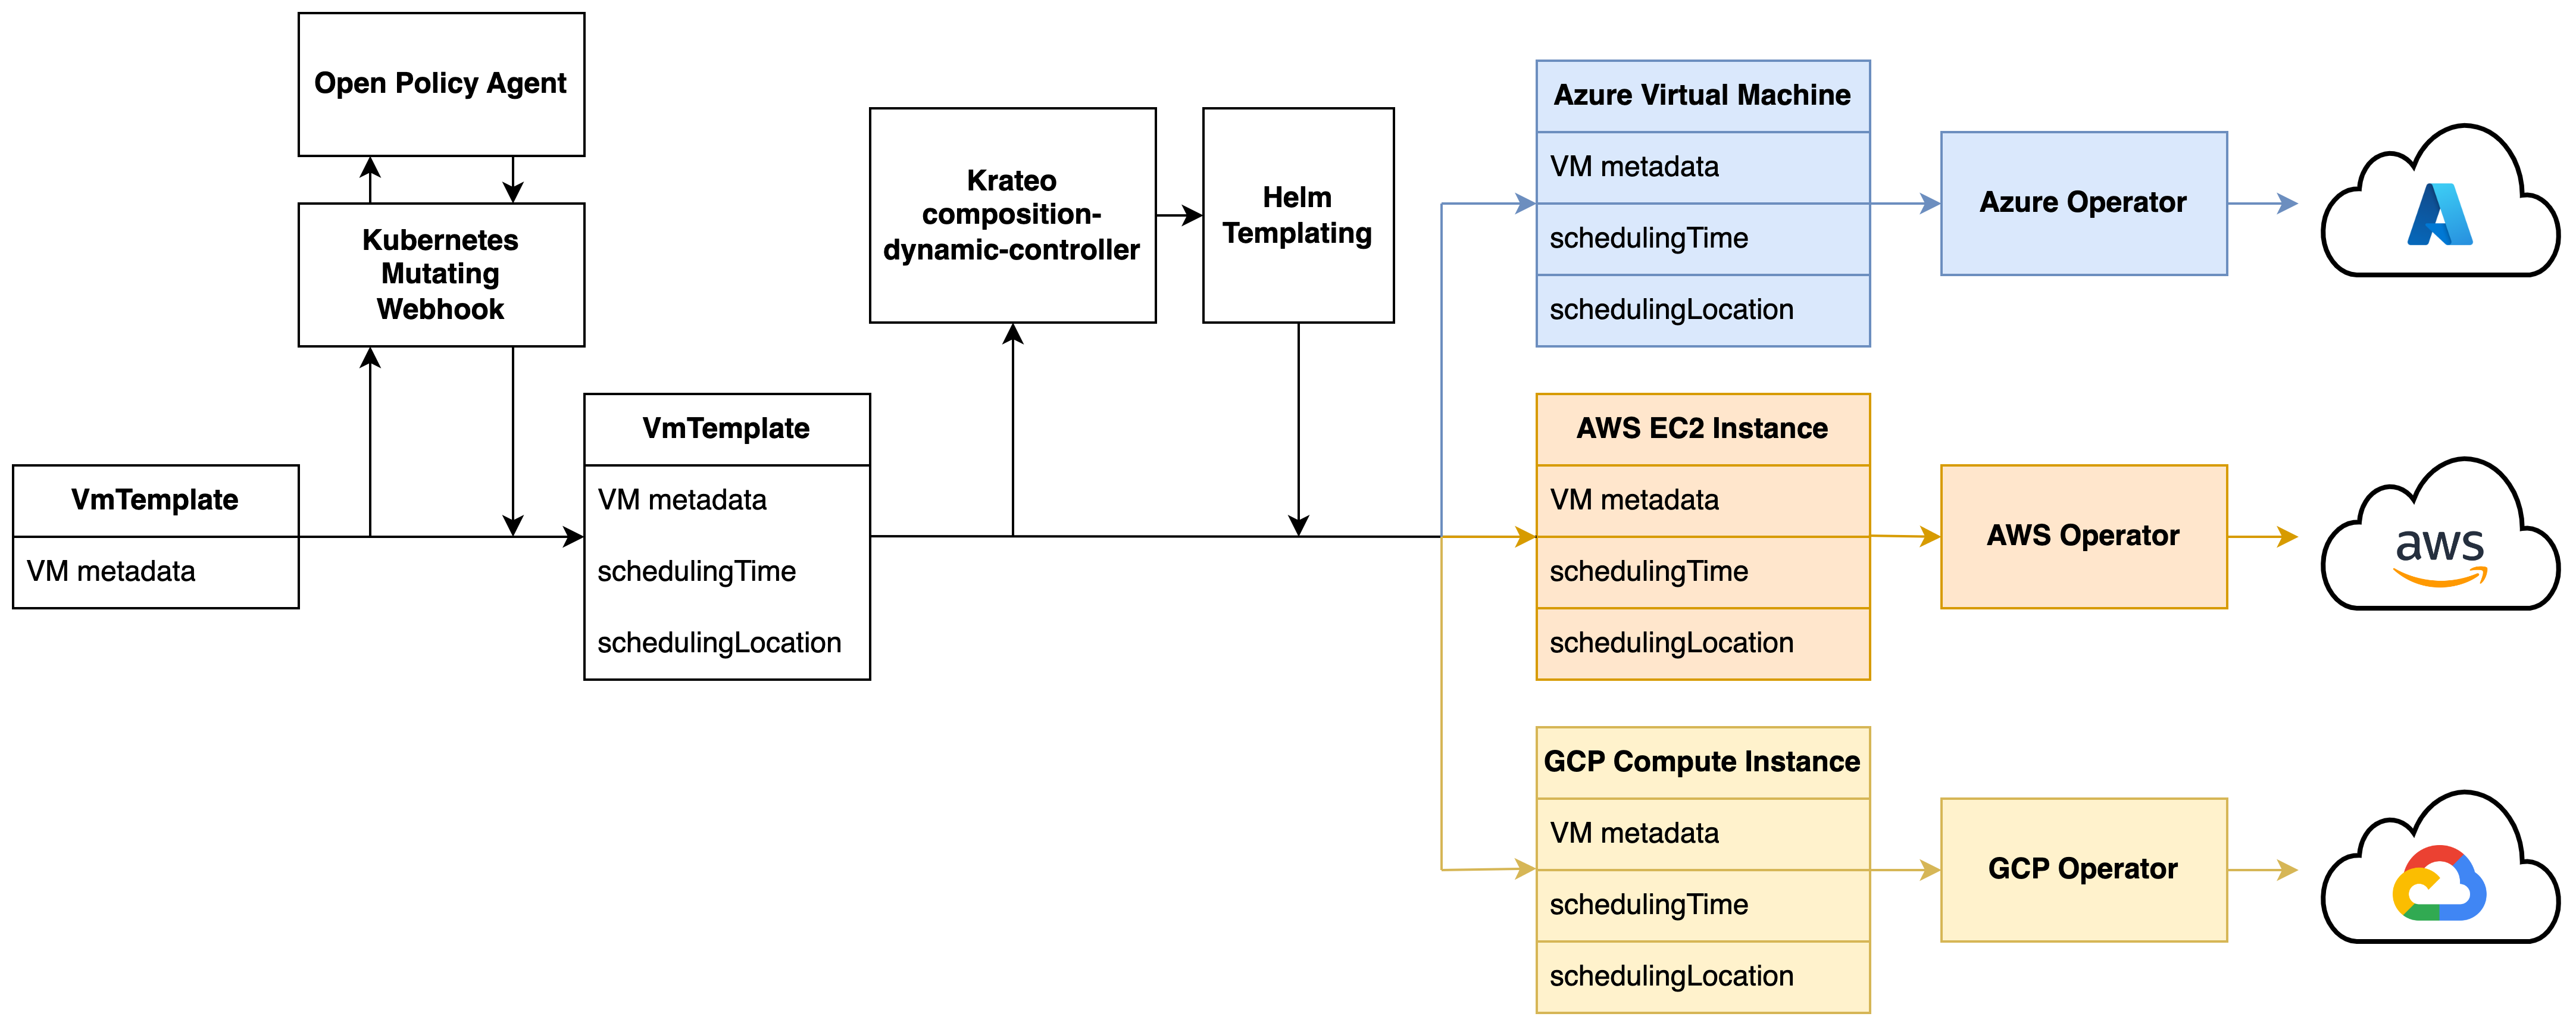
\includegraphics[width=1\linewidth]{images/operators.png}
\caption{Multi-cloud resource management through Kubernetes operators}
\label{fig:operators}
\end{figure}

\newpage

\subsection{Azure Kubernetes Operator}

Microsoft Azure provides a Kubernetes operator called \textbf{Azure Service Operator v2} (ASO).
Currently, ASO supports more than 150 different Azure resources.
minimum set of resources needed for vm provisioning on Azure throgh Azure service operator is is:

\begin{itemize}[itemsep=0.2pt, topsep=1pt] \item[$\bullet$] Virtual Network 
\item[$\bullet$] Virtual Network Subnet
\item[$\bullet$] Network Interface
\item[$\bullet$] Virtual Machine
\end{itemize}

\begin{figure}[H]
\centering
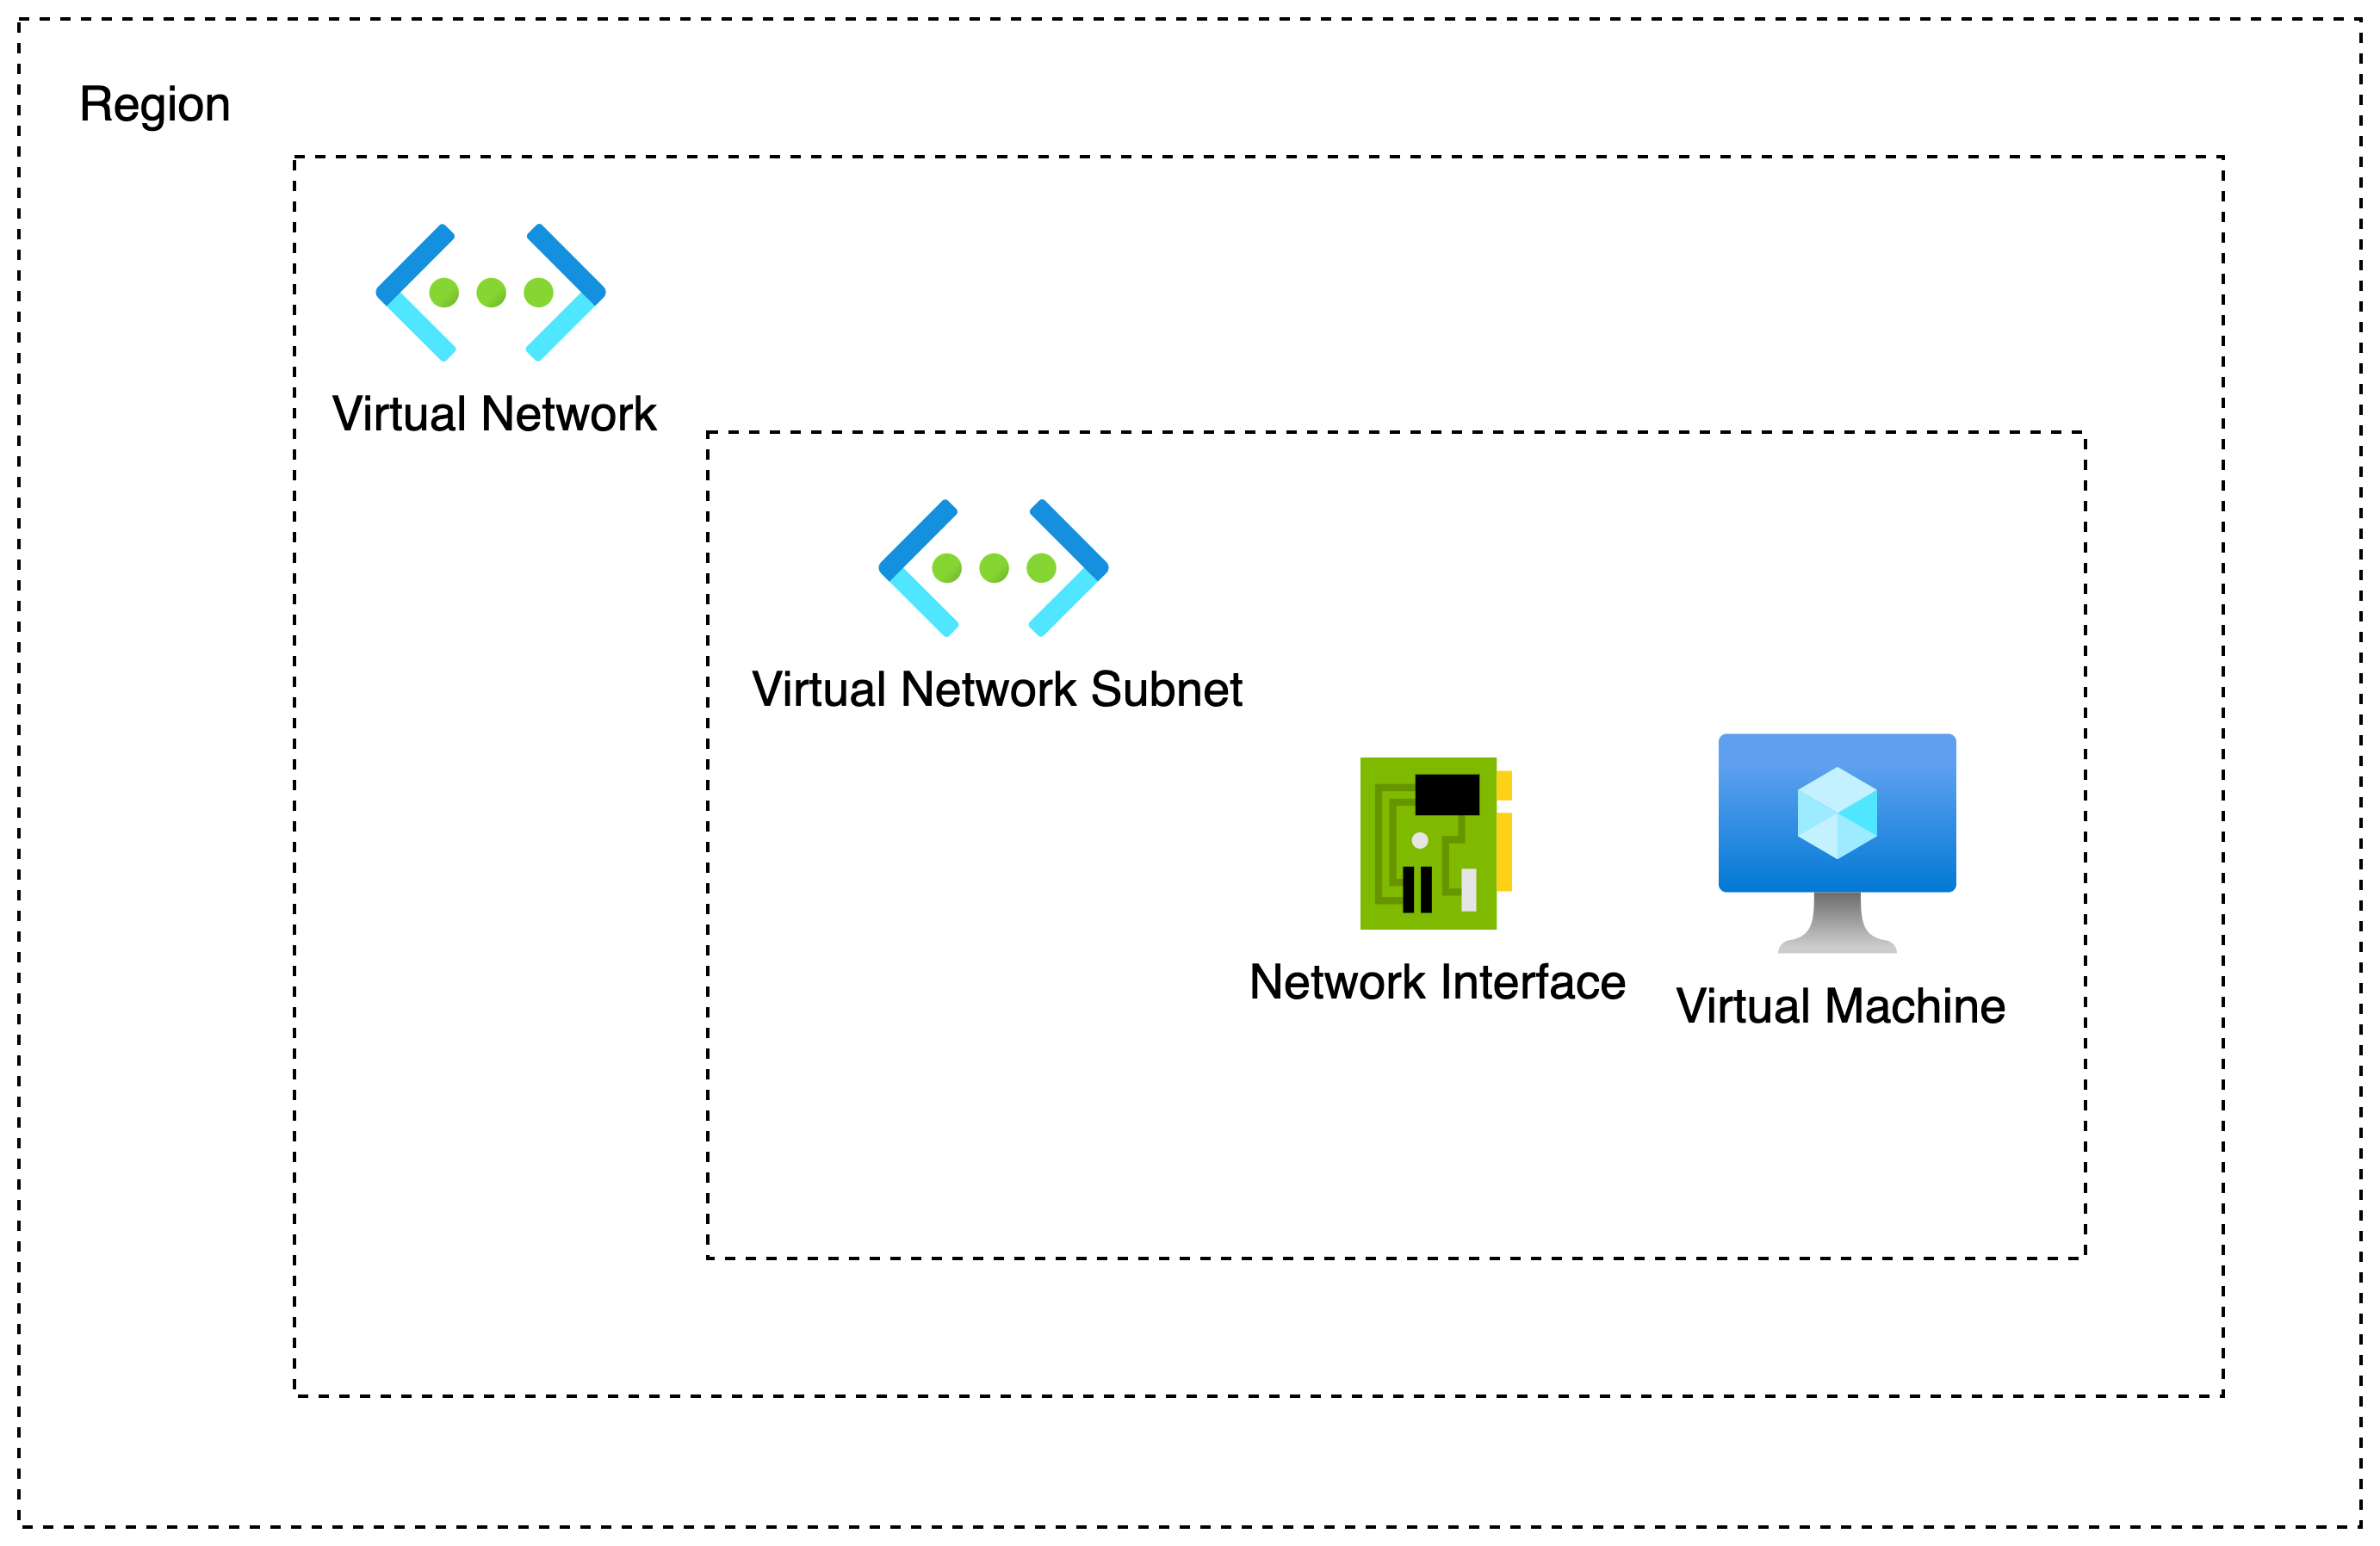
\includegraphics[width=0.75\linewidth]{images/azure.png}
\caption{Minimum set of Azure resources for VM provisioning}
\label{fig:azure}
\end{figure}






INSTANCE CR example











\subsection{GCP Operator}

minimum set of resources needed for vm deployment


\begin{figure}[H]
\centering
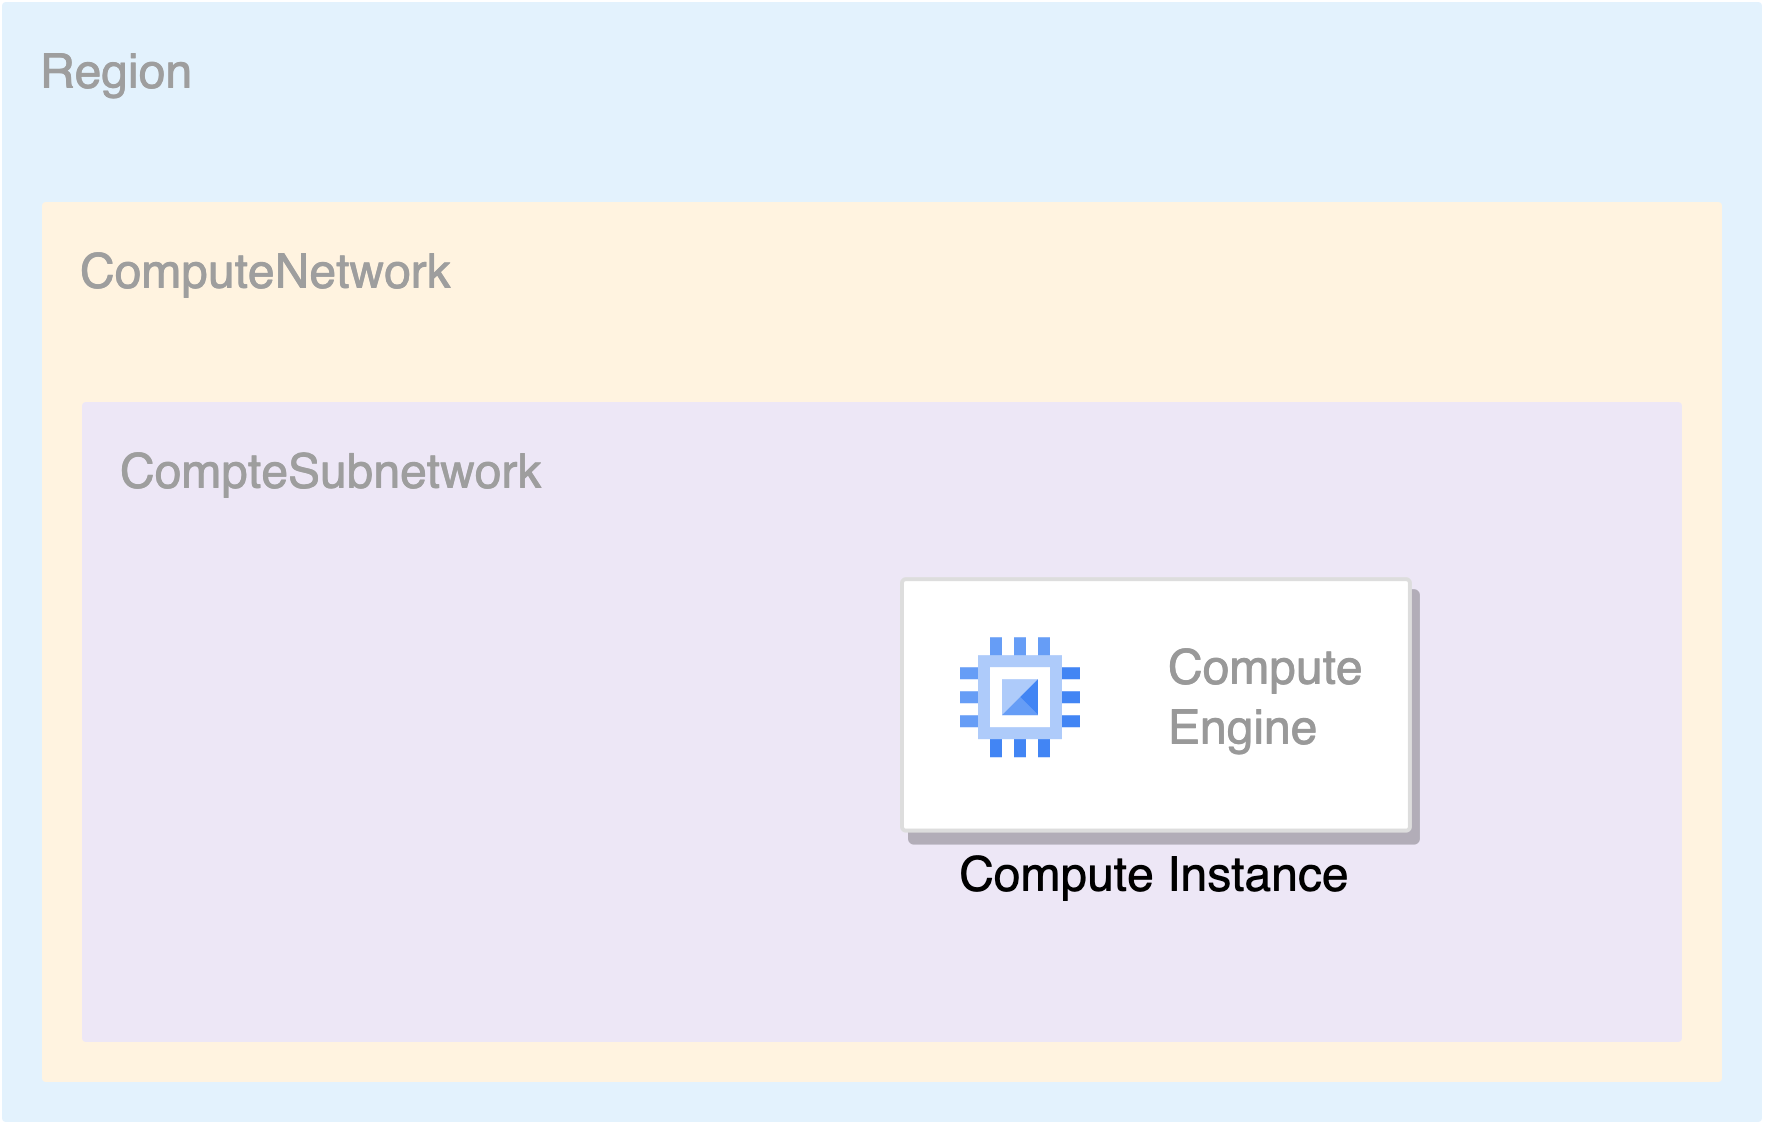
\includegraphics[width=0.75\linewidth]{images/gcp.png}
\caption{Minimum set of GCP resources for VM provisioning}
\label{fig:gcp}
\end{figure}




INSTANCE CR example

some fields are based on regions
some fields are based on zones


networkinterface is directly defined in the instance manifest,
no additional resource needed



\subsection{AWS Operator}

this is a collection of operators that are part of the AWS controllers for Kubernetes (ACK) project.

minimum set of resources needed for vm provisioning

\begin{itemize}[itemsep=0.2pt, topsep=1pt] 
\item[$\bullet$] VPC
\item[$\bullet$] Subnet
\item[$\bullet$] EC2 Instance
\end{itemize}






\begin{figure}[H]
\centering
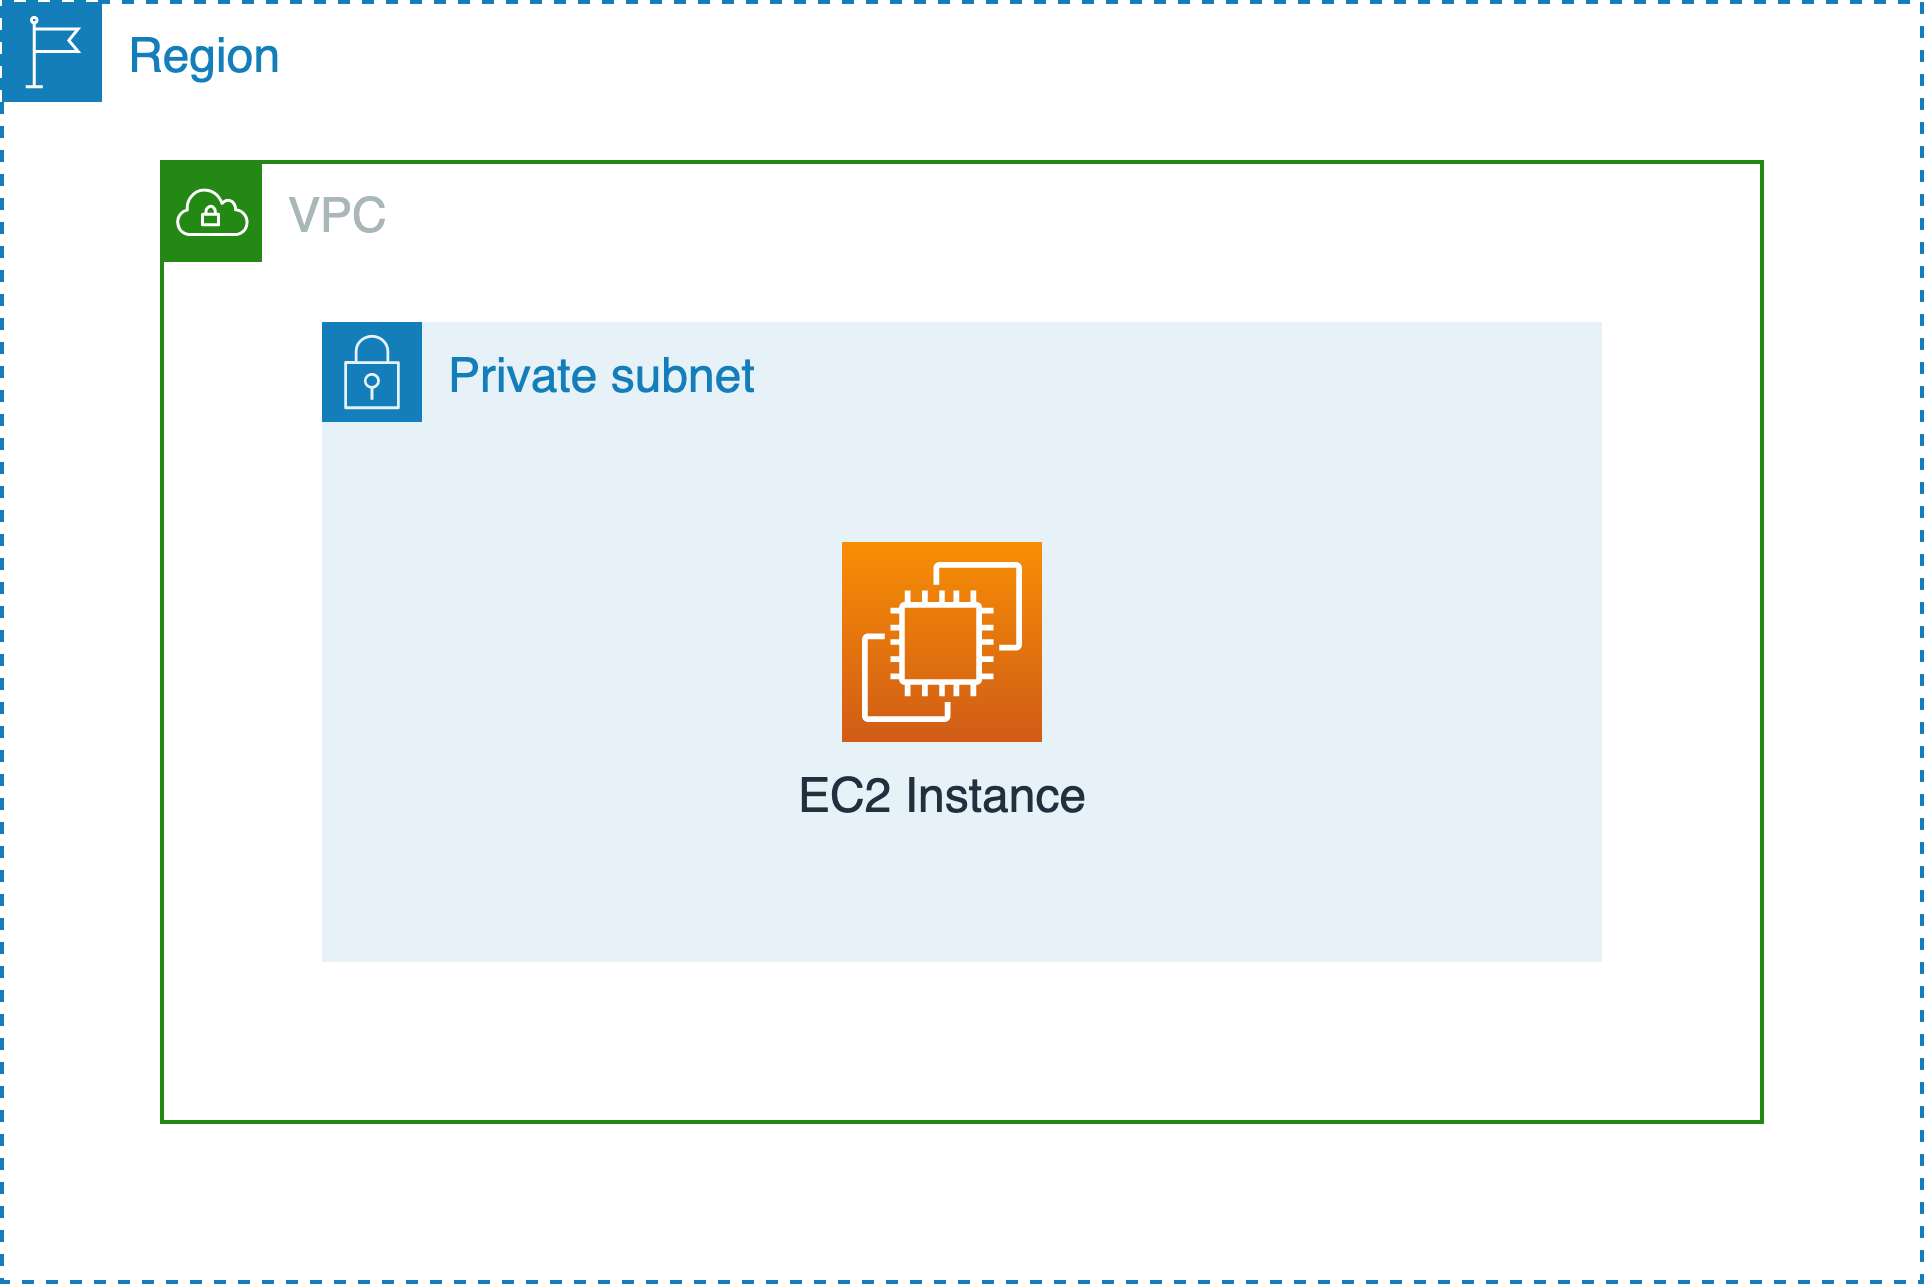
\includegraphics[width=0.75\linewidth]{images/aws.png}
\caption{Minimum set of AWS resources for VM provisioning}
\label{fig:aws}
\end{figure}


As described at the beginning of this section, the implementation approach adopted in our system ensures compatibility with diverse cloud provider design choices. Cloud providers may impose different constraints and best practices when managing Kubernetes-native resources, and the system is designed to adapt to these variations seamlessly.

One notable design choice observed with the AWS operator is the restriction on referencing some Kubernetes objects inside a Custom Resource (CR) manifest. This limitation means that developers cannot directly link a resource (e.g., a Virtual Machine) to another Kubernetes object (e.g., a Subnet) using built-in object references.

To overcome this limitation, our system leverages Helm’s lookup function, which dynamically retrieves Kubernetes object details at runtime. This method allows us to fetch required parameters without directly referencing Kubernetes objects in the CR, ensuring compatibility with the AWS operator’s design constraints. The following example demonstrates how the lookup function can be used to resolve subnet IDs dynamically and inject them into the CR manifest.

\begin{lstlisting}[language=yaml, caption={Helm Lookup Example: Dynamically Resolving Subnet IDs}, label={lst:helm_lookup}]
...
apiVersion: ec2.services.k8s.aws/v1alpha1
kind: Instance
metadata:
  name: {{ .Values.vmName }}
  namespace: {{ .Values.namespace | default "greenops" }}
...
spec:
  ...
  subnetID: {{ (lookup "ec2.services.k8s.aws/v1alpha1" "Subnet" (.Values.namespace | default "greenops") (printf "%s-subnet" .Values.vmName)).status.subnetID }}
...
\end{lstlisting}

In this example, the lookup function retrieves the subnet ID from a Subnet CR dynamically, based on the VM name and namespace. Then, the subnet ID is injected into the Instance CR manifest, ensuring that the VM is provisioned in the correct subnet.

An example by AWS Operator where instead a direct reference to a resource is allowed is the following:

\begin{lstlisting}[language=yaml, caption={Helm Lookup Example: Dynamically Resolving Subnet IDs}, label={lst:helm_lookup}]
...
apiVersion: ec2.services.k8s.aws/v1alpha1
kind: Subnet
metadata:
  name: {{ .Values.vmName }}-subnet
  namespace: {{ .Values.namespace | default "greenops" }}
...
spec:
  vpcRef: 
    from: 
      name: {{ .Values.vmName }}-vpc
      namespace: {{ .Values.namespace | default "greenops" }}
...
\end{lstlisting}

In this case, the Subnet CR manifest directly references the VPC CR using name and namespace since the Operator is designed to support this type of relationship.


---

Amazon
AMI
what is an AMI
what are the parameter to determine an AMI

Testing:
manual tests were made to check correspondance from scraped ubuntu website and AWS console.


\newpage

\section{Open Policy Agent (OPA)}

Open Policy Agent (OPA) is an open-source general-purpose \textbf{policy engine} that enables unified policy enforcement across cloud-native environments. OPA provides a declarative language called Rego enabling a paradigm known as ``\textbf{Policy as Code}" \cite{opa_docs}.

Open Policy Agent can be integrated as a sidecar container, host-level daemon, or library to perform policy decisions for a plethora of use cases: microservices, Kubernetes admission control, CI/CD pipelines,  API gateways and more \cite{opa_docs}. 

\subsection{Policy as Code paradigm}

According to AWS, Policy-as-Code (PaC) is a software automation approach which is similar to Infrastructure-as-Code (IaC) \cite{pac_aws}. PaC helps assess company system configurations and validate compliance requirements through software automation \cite{pac_aws}. The perceived value of this type of automation in the software development lifecycle has grown significantly in modern enterprises. This large adoption is probably driven by the inherent consistency and reliability it provides, ensuring standardized enforcement of policies and reducing human error \cite{pac_aws}.

OPA's generic defintion of policy is: ``\textit{A policy is a set of rules that governs the behavior of a software service}" \cite{opa_philosophy}. OPA provides a high-level declarative language called \textbf{Rego} to define policies in a flexible manner. One of OPA's key strengths is its \textbf{domain-agnostic design}, allowing it to enforce policies across various systems and environments. This makes it highly adaptable to different use cases, ranging from access control to infrastructure security. Some representative examples of policies that OPA can enforce include:

\begin{itemize}[itemsep=0.2pt, topsep=1pt] \item[$\bullet$] Restricting which image registries can be used for deploying new Pods in a Kubernetes cluster.
\item[$\bullet$] Controlling whether a specific user is permitted to perform delete operations on certain resources.
\item[$\bullet$] Enforcing network security policies, such as blocking external access to sensitive services.
\item[$\bullet$] Ensuring infrastructure compliance, for example, by verifying that new cloud resources to be provisioned follow predefined security configurations.
\item[$\bullet$] Enforcing that new deployed servers must have the prefix ``server-" in their name.
\end{itemize}
Therefore, the use cases covered span from role-based access control to container image security and beyond.
\newline


Another important aspect of OPA is that it effectively \textbf{decouples} policy decision-making from policy enforcement, enabling organizations to implement consistent and scalable authorization across their distributed systems \cite{test}.
In practice, this means that when a software module needs to make a policy decision, it queries OPA, supplying relevant data as input. In other words, policy decisions are \textbf{offloaded} to OPA rather than being hardcoded within individual services. This approach offers several key advantages:
\begin{itemize}[itemsep=0.2pt, topsep=1pt]
  \item[$\bullet$] \textbf{Centralized policy management}: policies are defined in a single location, ensuring uniform enforcement across all services.
  \item[$\bullet$] \textbf{Improved maintainability}: updating policies does not require modifying, recompiling or redeploying application code, reducing complexity and deployment overhead.
  \item[$\bullet$] \textbf{Greater flexibility}: policies can be dynamically updated (e.g., with CI/CD approaches) based on evolving security and compliance requirements 
  \item[$\bullet$] \textbf{Scalability}: since OPA and application modules are not tightly coupled.
\end{itemize} 




\subsection{OPA architecture overview}

As mentioned in the introduction to this section, one common approach to integrating OPA into a software system is by deploying it as a host-level daemon. The latter is essentially a lightweight server that processes policy queries via HTTP requests. This setup allows services to offload policy decision-making to OPA in a scalable and efficient manner since the two entities are not tighlty coupled.

A standard OPA deployment consists of three main components:

\begin{itemize}[itemsep=0.2pt, topsep=1pt]
\item[$\bullet$] \textbf{OPA Server} – The core service that evaluates policy queries and returns decisions based on defined rules, contextual data and input data.
\item[$\bullet$] \textbf{OPA Policies} – Rules written in the Rego language that define the logic to be enforced.
\item[$\bullet$] \textbf{Data} – Optional contextual information, typically structured in JSON format, that policies use to make informed decisions along with input data.
\end{itemize}

To facilitate deployment and management, Rego policies and associated contextual data are packaged into \textbf{policy bundles}, as described in section \ref{sec:opa_policies}. These bundles enable version-controlled, centralized policy distribution, ensuring consistency and maintainability across distributed environments. \newline


\begin{figure}[htb]
\centering
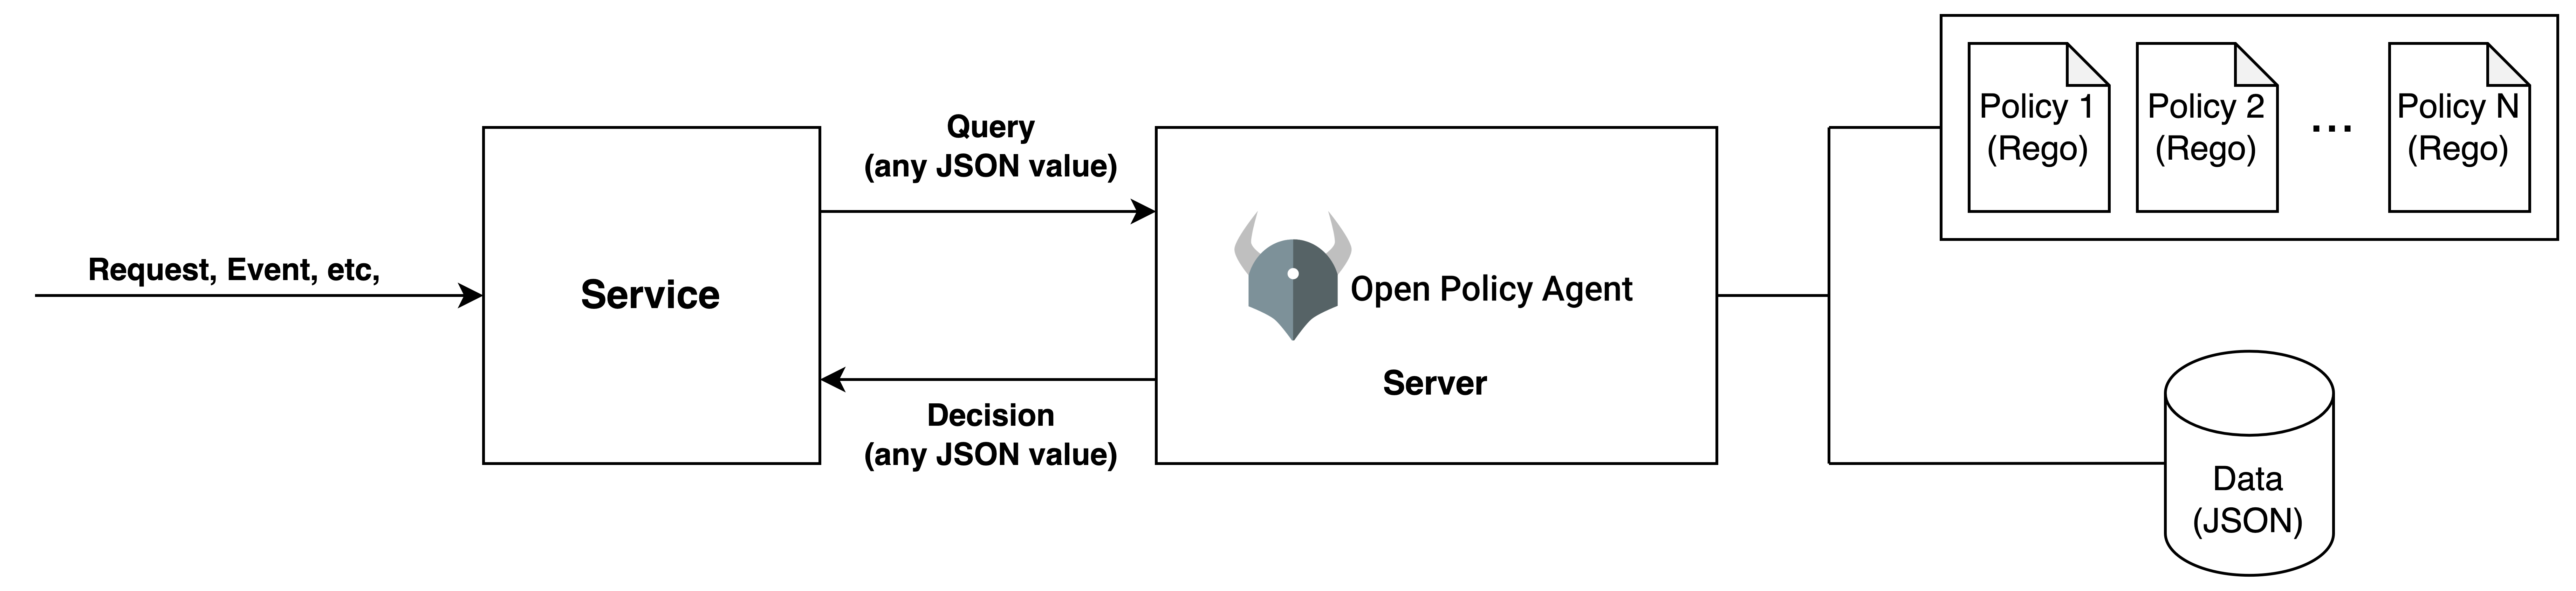
\includegraphics[width=1\linewidth]{images/OPA.png}
\caption{OPA architecture}
\label{fig:opa_architecture}
\end{figure}


OPA accepts arbitrary structured data as input.
and  Like query inputs, your policies can generate arbitrary structured data as output.

\subsection{OPA and external data}

types of external data strategies

http.send()
paramters 



\subsection{OPA integration with Kubernetes}

In Kubernetes admission control, policy enforcement is handled by the \textbf{Kubernetes API server} itself. OPA makes the policy decisions when queried by the admission controller, but the actual enforcement (namely allowing or denying requests) is executed by Kubernetes' built-in admission control mechanisms. This workflow is represented in figure \ref{fig:webhook_opa} where \textbf{AdmissionrReview request} and \textbf{AdmissionReview response} are respectively input and output of the whole OPA section. The API Server sends the entire Kubernetes object in the webhook request to OPA. %cite OPA kubernetes primer
The Kubernetes API server will use the received AdmissionReview response for its decision. \\
%\cite{opa_philosophy}


\begin{figure}[htb]
\centering
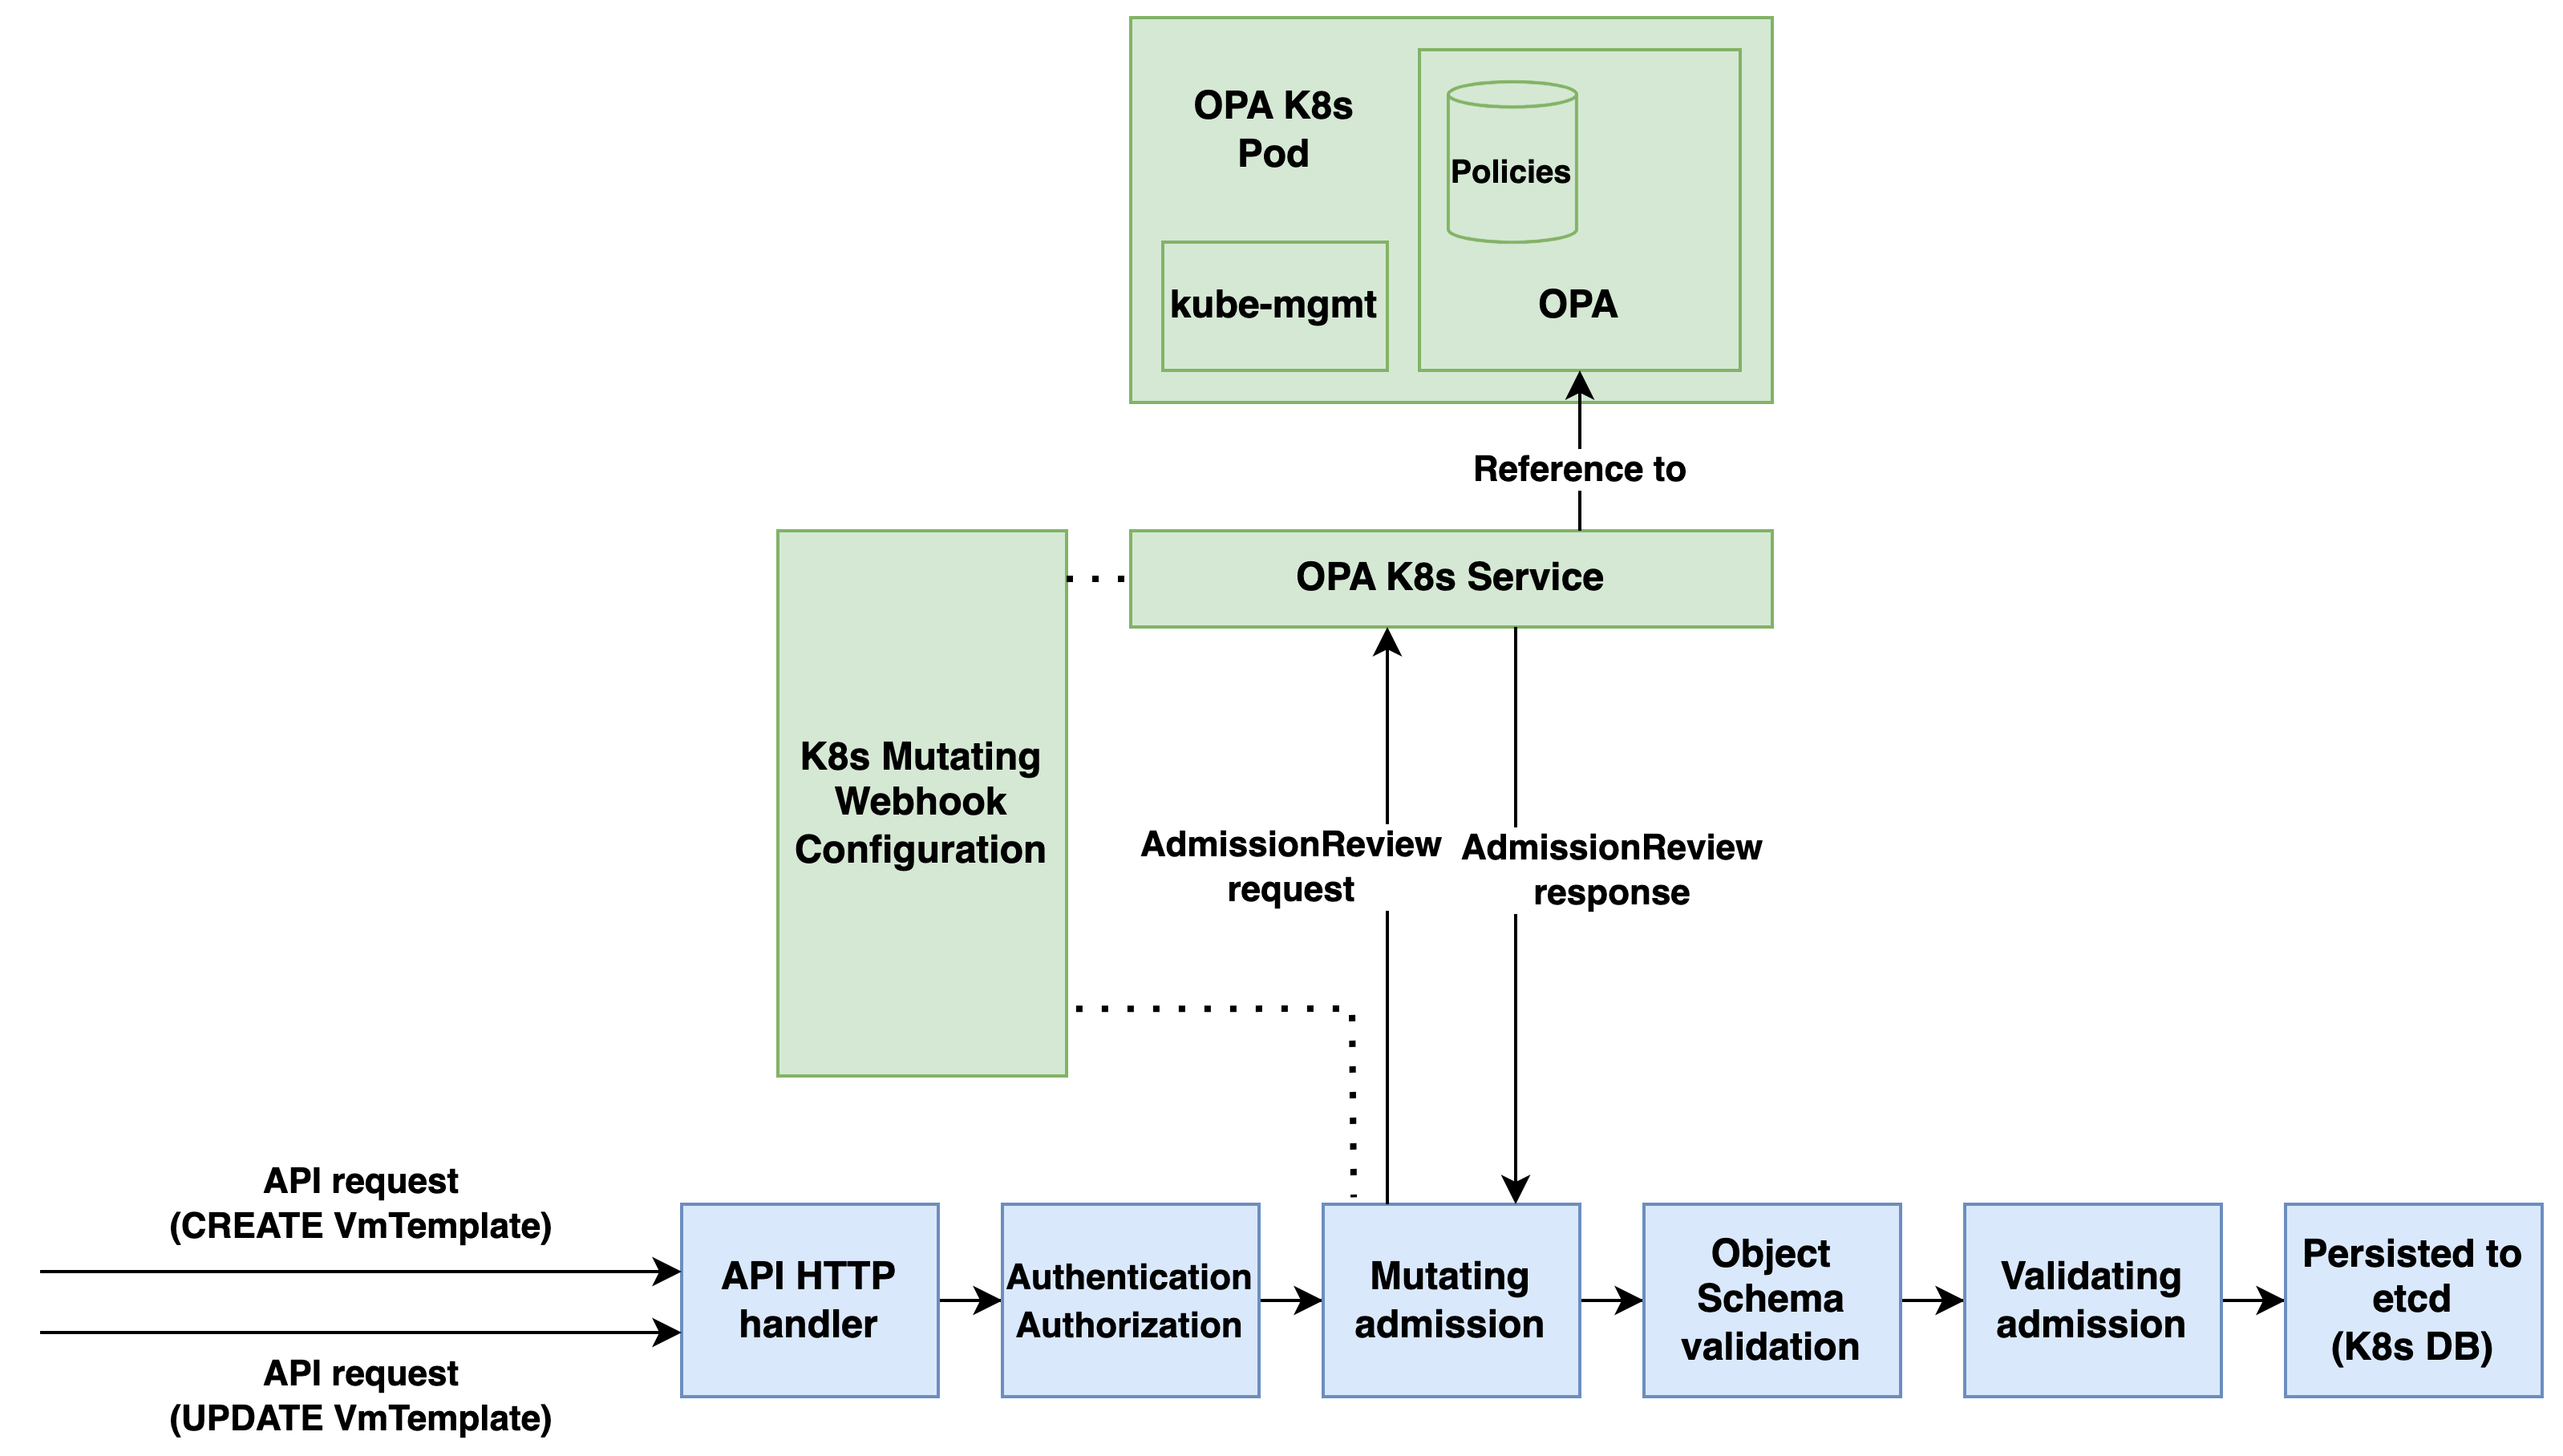
\includegraphics[width=1\linewidth]{images/webhook.png}
\caption{Kubernetes mutating webhook and OPA integration}
\label{fig:webhook_opa}
\end{figure}



In a Kubernetes deployment, an OPA Pod typically consists of the following containers:
\begin{itemize}[itemsep=0.2pt, topsep=1pt]
  \item[$\bullet$] OPA server container
  \item[$\bullet$] \textbf{kube-mgmt} container \\
\end{itemize} 

kube-mgmt functions as a \textbf{sidecar container} within a Kubernetes Pod. The sidecar container pattern is a common Kubernetes design paradigm in which auxiliary containers run alongside the main application container within the same Pod. These additional containers serve to enhance, extend, or support the primary application's functionality without modifying its core logic.  % cite https://kubernetes.io/docs/concepts/workloads/pods/sidecar-containers/
The primary responsibility of kube-mgmt is to replicate Kubernetes resources into the OPA instance (OPA container). This operation is essential for OPA to access and evaluate policies based on real-time cluster state, enabling dynamic policy enforcement. By synchronizing these resources, kube-mgmt ensures that OPA has an up-to-date view of relevant Kubernetes objects.
This is especially useful to enforce policies that deals with name conflicts, where OPA needs to check existing names in the cluster for the decision.
Additionally, it allows for loading policies directly from the Kubernetes cluster by retrieving them in the form of ConfigMaps. This feature is particularly useful when policies need to be dynamically updated based on the current state of the cluster. However, in the system described in this thesis, this latter feature is not employed in the current implementation. %cite https://github.com/open-policy-agent/kube-mgmt


In the current system configuration, the kube-mgmt container is deployed to facilitate resource replication, ensuring that Kubernetes resources, including CustomResourceDefinitions (CRDs), are synchronized with the OPA instance. However, at present, no policies require interrogation of VmTemplate resources that are already present in the system.
Looking ahead, future policies could leverage VmTemplate resource information to enforce naming conflict resolution, quota management, or additional constraints.



\newpage




\subsection{OPA policies}
\label{sec:opa_policies}

%example of a policy:
%(https://www.openpolicyagent.org/docs/latest/kubernetes-primer/)





As OPA official documentation describes, when the Kubernetes AdmissionReview request from the webhook arrives, it is binded to the input document and generates the default, ``root", decision: \textit{system.main}
%\cite

The root policy is responsible for generating the AdmissionReview response in accordance with the Kubernetes API specifications. It is the duty of the policy developer to write Rego code that produces a well-formed AdmissionReview response, ensuring that the OPA server can then correctly communicate its decision to the Kubernetes admission controller.
%cite



It is deemed useful to show one of the simplest and common example of a OPA policy in the \textbf{Kubernetes admission control context}. That is: to ensure all images for Kubernetes Pods come from a trusted registry, namely \textit{unitn.it}. \\


It is important to note that, in this case, due to the simplicity of the policy, no additional contextual data in JSON format is required.


policy compilation
policy are compiled
compile time errors like merge errors if data is clashing for instance



\begin{comment}
    \lstset{
   language=Go,
   basicstyle=\ttfamily\small,
   breaklines=true,
   showstringspaces=false,
   commentstyle=\color{green!60!black},
   keywordstyle=\color{blue},
   stringstyle=\color{purple},
   numberstyle=\tiny,
   numbers=left,
   backgroundcolor=\color{gray!10},
   frame=single,
   captionpos=b
}
\end{comment}


\begin{lstlisting}[language=Rego, caption={Rego policy for Pods registry},
label=lst:rego_data_mapping]
                                          
deny contains msg if {                                                      
    input.request.kind.kind == "Pod"                                        
    image := input.request.object.spec.containers[_].image                  
    not startswith(image, "unitn.it/")                                     
    msg := sprintf("image '%v' comes from untrusted registry", [image])     
}
\end{lstlisting}

\begin{lstlisting}[caption={Rego ``root" policy (system.main)}]
package system

import data.kubernetes.admission

main := {
	"apiVersion": "admission.k8s.io/v1",
	"kind": "AdmissionReview",
	"response": response,
}

default uid := ""

uid := input.request.uid

response := {
	"allowed": false,
	"uid": uid,
	"status": {"message": reason},
} if {
	reason := concat(", ", admission.deny)
	reason != ""
}

else := {"allowed": true, "uid": uid}
\end{lstlisting}


\newpage
\lstset{style=jsonstyle}
\begin{lstlisting}[caption={AdmissionReview request}]
{
    "apiVersion": "admission.k8s.io/v1",
    "kind": "AdmissionReview",
    "request": {
        "kind": {
            "group": "",
            "kind": "Pod",
            "version": "v1"
        },
        "object": {
            "metadata": {
                "name": "myapp"
            },
            "spec": {
                "containers": [
                    {
                        "image": "bitnami/node:22",
                        "name": "nodejs"
                    }
                ]
            }
        }
    }
}
\end{lstlisting}


\lstset{style=jsonstyle}
\begin{lstlisting}[caption={AdmissionReview response}]
{
    "apiVersion": "admission.k8s.io/v1",
    "kind": "AdmissionReview",
    "response": {
        "allowed": false
        "status": {
            "message": "image 'bitnami/node:22' comes from untrusted registry"
        }
    }
}
\end{lstlisting}

Therefore, in this specific case, the creation of the Kubernetes Pod will be denied. OPA is responsible for \textbf{decision-making}, determining that the request do not complies with the defined policies, while the Kubernetes API server handles \textbf{policy enforcement}, effectively rejecting the CREATE request since it violates the specified rules.


\subsection{OPA Policy bundles}

what is a policy bundle

how to package a bundle
budles as OCI images

OPA server is configured to pull bundles from a specified registry repository
1 or more bundles

CI CD
gitops



descrizione release.yml

impacchettamento policy






hot reload performed at application level 
no need for the opa K8s pod to be restarted

big advantage since if we want to add a new policy or update data we just push those changes in a code repository (like on GitHub) and the CI/CD (GitHub action) will bundle and publish the policies as a OCI Container on a Container registry. \newpage


\begin{figure}[htb]
\centering
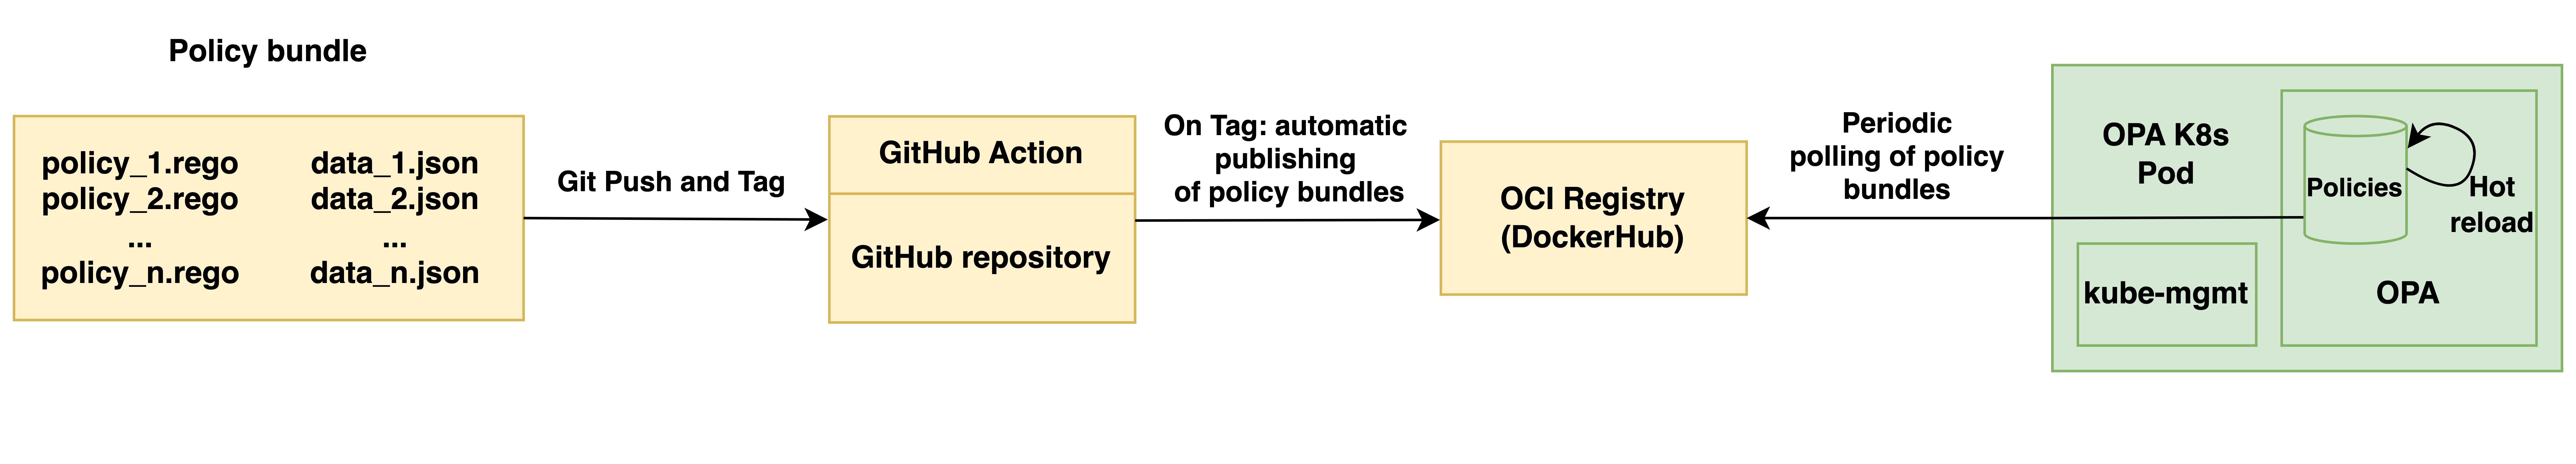
\includegraphics[width=1\linewidth]{images/opa_bundles.png}
\caption{OPA bundles}
\label{fig:opa_bundles}
\end{figure}


\subsection{OPA Gatekeeper}

%(what is opa gatekeeper)
OPA Gatekeeper is ... could be seen as the go-to solution for kuberntes architecture.
this is prbably true for simple use cases. not useful for the problem that must be tackled in this system (mutation and leveraging external data). differences wrt normal OPA deployment. OPA Gatekeeper advantages: no policy bundles but K8s custom resources (name of the CR to be added). for basic mutations is also fasibile and in this case rego code in not needed (there are specific resource called mutators with specific fields to tune in order to modify specific resource fields). OPA Gatekeeper limitations: on mutations and external data





To illustrate the differences between a standard OPA policy and an OPA Gatekeeper policy, we present two examples:  
(1) a simple Rego policy that enforces a basic constraint, and  
(2) the corresponding policy implemented as an OPA Gatekeeper \textbf{ConstraintTemplate} and \textbf{Constraint} Kubernetes resources.

The first example demonstrates a standalone **Rego policy**, which can be evaluated directly by an OPA instance. While this approach is flexible and allows for fine-grained policy definition, it requires manual integration into the system, including policy distribution and enforcement setup.  

\begin{lstlisting}[language=rego, caption={Simple OPA Rego Policy}, label={lst:opa-rego}]
package kubernetes.admission

deny[msg] {
  input.request.kind.kind == "Pod"
  input.request.object.metadata.namespace == "restricted"
  msg := "Pods cannot be created in the 'restricted' namespace."
}
\end{lstlisting}

The second example utilizes OPA Gatekeeper, which extends OPA with Kubernetes-native Custom Resource Definitions (CRDs), enabling declarative policy management. By using a ConstraintTemplate, policies can be enforced dynamically through Kubernetes, making them easier to distribute and manage.
In other words, with this kind of setting, OPA policy bundles are not employed.

\begin{lstlisting}[language=yaml, caption={OPA Gatekeeper ConstraintTemplate}, label={lst:gatekeeper-template}]
apiVersion: templates.gatekeeper.sh/v1
kind: ConstraintTemplate
metadata:
  name: podnamespaceconstraint
spec:
  crd:
    spec:
      names:
        kind: PodNamespaceConstraint
  targets:
    - target: admission.k8s.gatekeeper.sh
      rego: |
        package kubernetes.admission
        deny[msg] {
          input.review.object.metadata.namespace == "restricted"
          msg := "Pods cannot be created in the 'restricted' namespace."
        }
\end{lstlisting}

\begin{lstlisting}[language=yaml, caption={OPA Gatekeeper Constraint}, label={lst:gatekeeper-constraint}]
apiVersion: constraints.gatekeeper.sh/v1beta1
kind: PodNamespaceConstraint
metadata:
  name: restrict-namespace
spec:
  match:
    kinds:
      - apiGroups: [""]
        kinds: ["Pod"]
  parameters: {}
\end{lstlisting}







\subsection{Latency policy}

A representative example of a policy aligned with Service Level Objectives (SLOs) or Service Level Agreements (SLAs) is the latency policy described in this section.
Given an \textbf{origin region} and a \textbf{maximum latency threshold} (expressed in milliseconds), the objective is to determine a \textbf{set of eligible regions} where the inter-regional latency between the origin and each region in the set is equal to or below the specified threshold.
Enforcing such constraints helps mitigate the so-called ``\textbf{black hole phenomenon}" in the GreenOps use case, where all virtual machines (VMs) would otherwise be scheduled in a region with generally low carbon intensity, without considering additional constraints or performance requirements. By incorporating similar performance-aware policies, organizations can achieve a balance between environmental impact, performance, and service reliability.
The proposed flexible system enables organizations to fine-tune these factors according to their specific requirements or those of their users. 
This policy demonstrates the flexibility of OPA in handling diverse compliance scenarios. It is the responsibility of the policy developer to design an appropriate strategy for encoding relevant information into \textbf{well-structured JSON data models}, e.g., a latency matrix. Proper structuring ensures efficient policy evaluation, maintainability and extendability.






[figure of latency matrix (maybe 10x10?) with colors]



[code of the policy]



\lstset{style=jsonstyle}
\begin{lstlisting}[caption={Latancy matrix example}, label={lst:latency_matrix_example}]
...
"italynorth": {
                "australiacentral": 286,
                "australiacentral2": 278,
                "australiaeast": 279,
                "australiasoutheast": 266,
                ...
                "francecentral": 24,
                "francesouth": 15,
                "germanynorth": 25,
                "germanywestcentral": 20,
                "israelcentral": 50,
                "italynorth": 0,
                ...
},
"japaneast": {
                "australiacentral": 108,
                "australiacentral2": 107,
                "australiaeast": 104,
                "australiasoutheast": 115,
                "brazilsouth": 278,
                "canadacentral": 159,
                "canadaeast": 169,
                "centralindia": 122,
                "centralus": 137,
                "eastasia": 52,
                "eastus": 170,
                "eastus2": 163,
                ...
},
...
\end{lstlisting}

\subsection{GDPR policy}


Another policy configured is the GDPR


set of cloud regions that resides inside countries of the European Union.

speicifc regions for each cloud provider
encoded in the data in json (along with latency matrix)

\subsection{Mutation policy}

main policy
dedicated to 


patch code

emcopded patches


\subsection{Data mapping}

OPA is powerful enough to ...


this mappings are needed since the scheudler knows only...

inside the policy is a good place to do this mapping


\begin{figure}[H]
  \centering
  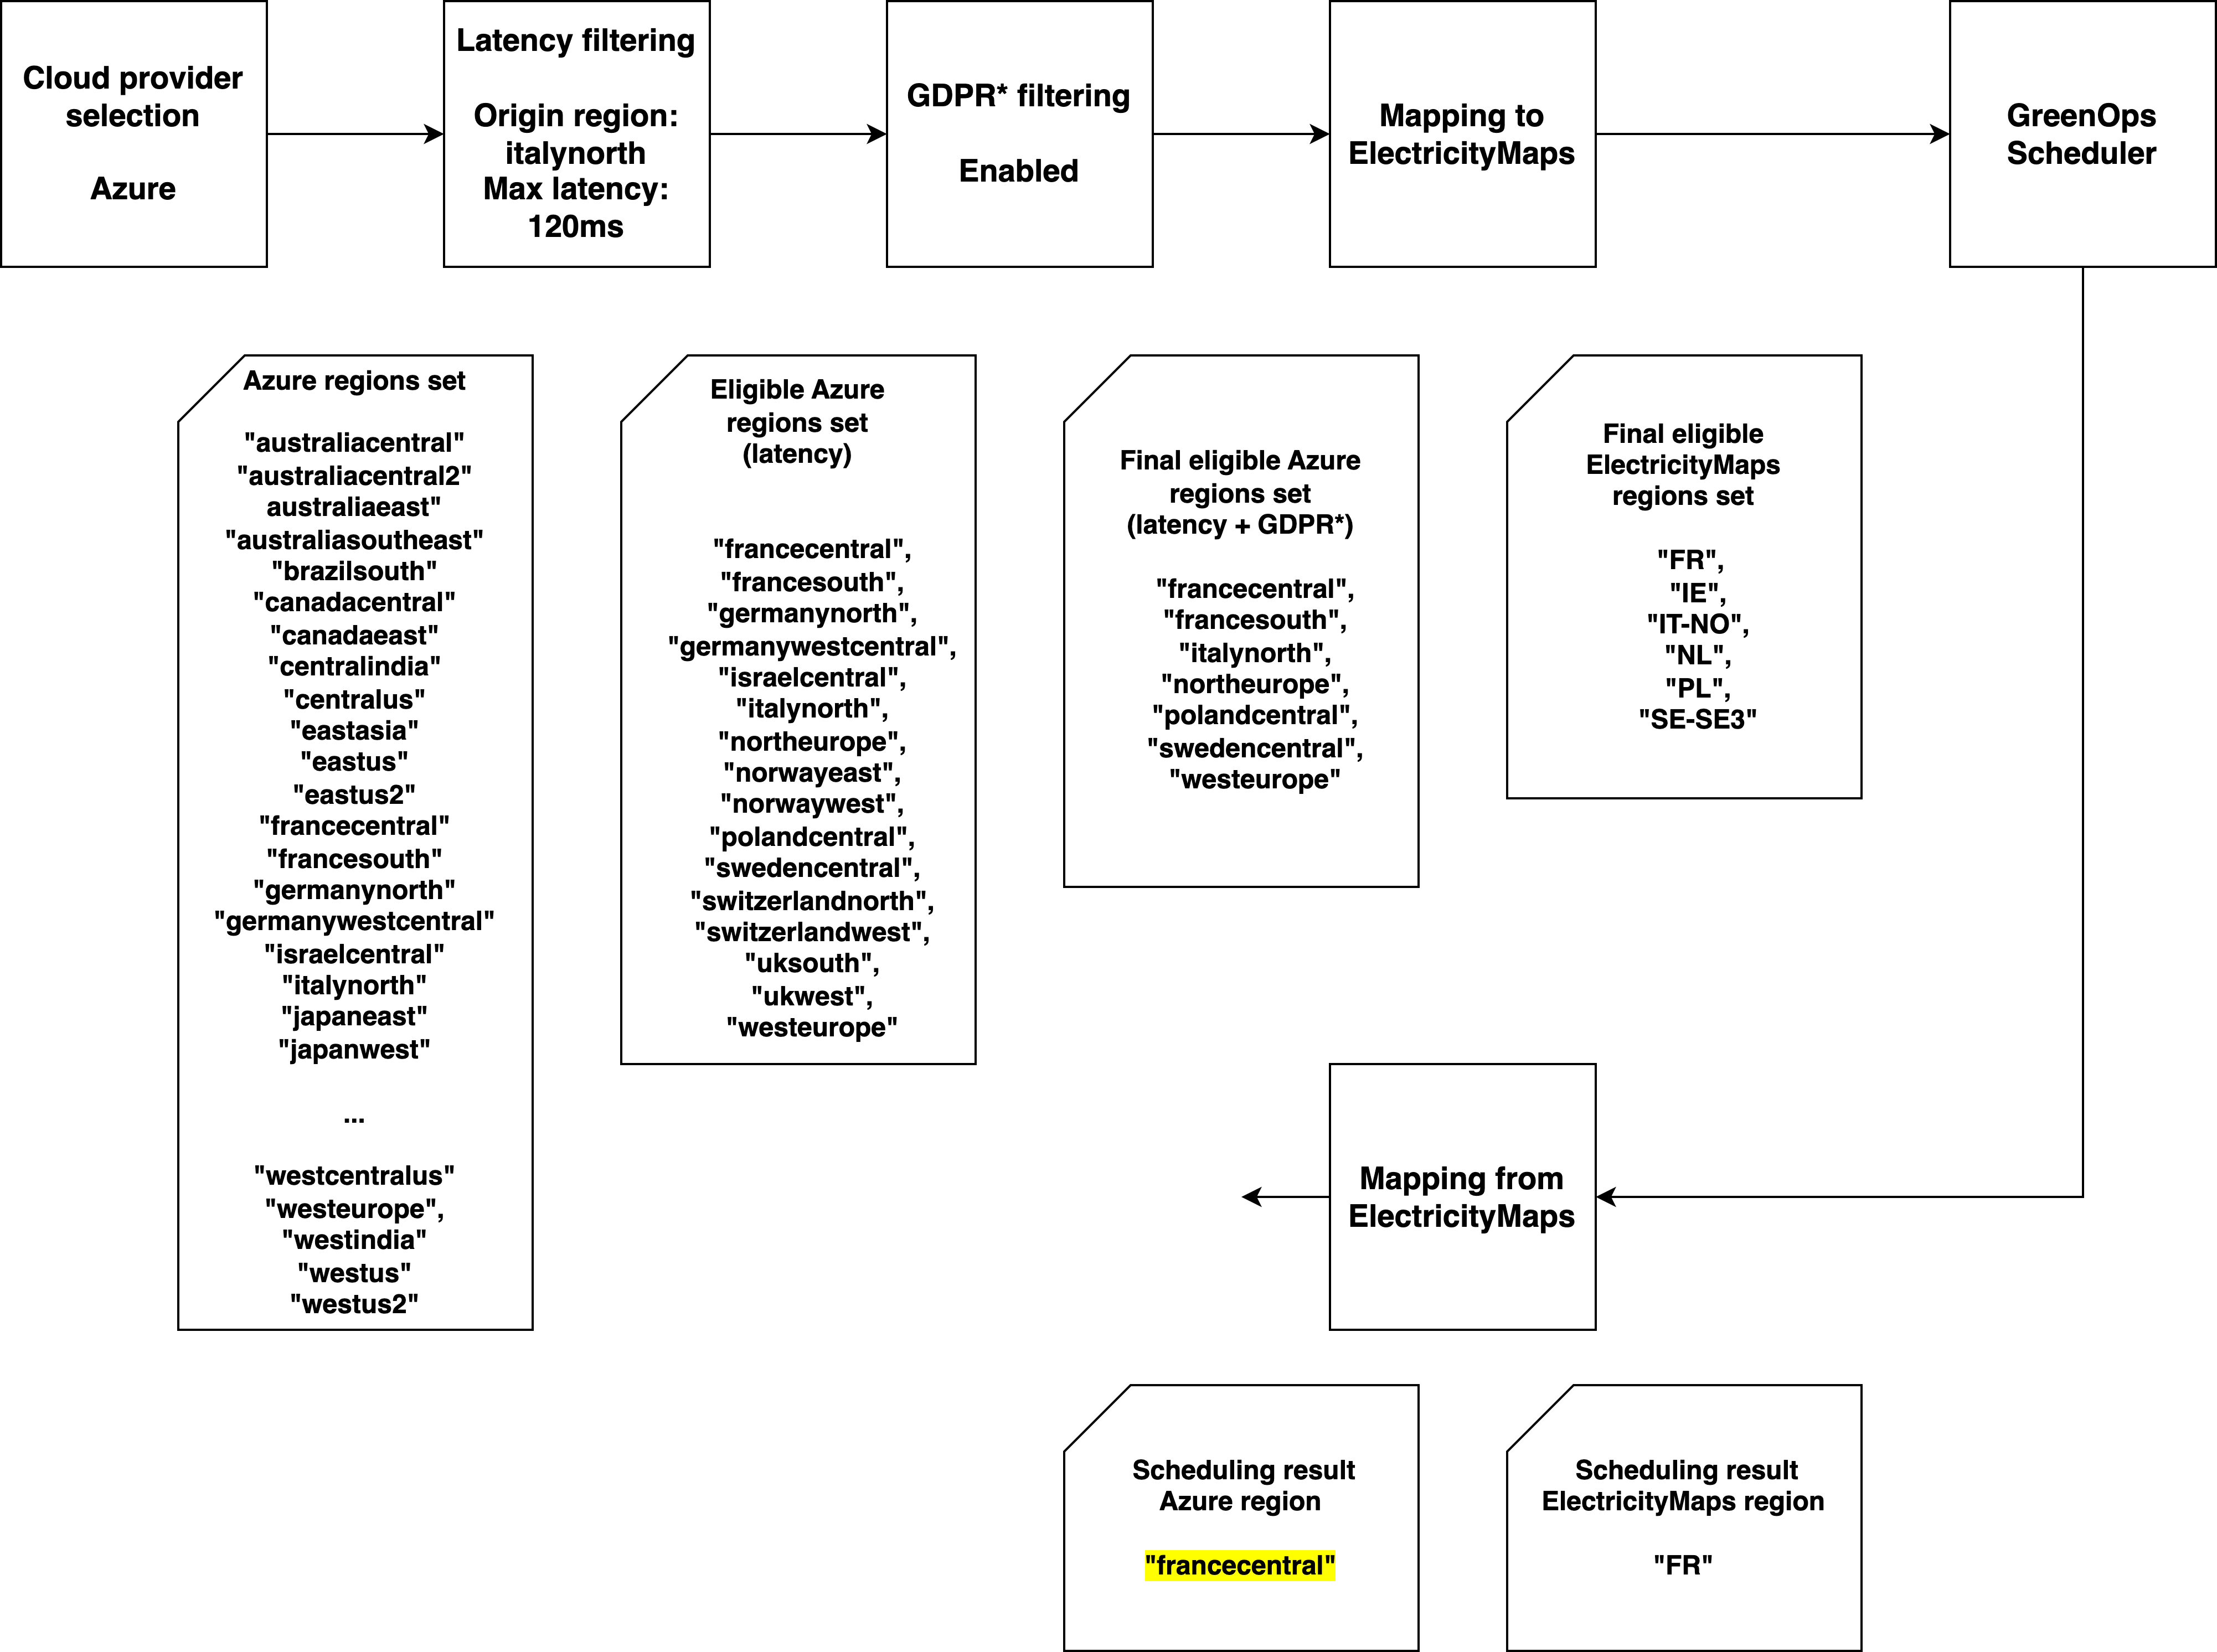
\includegraphics[width=1\linewidth]{images/data_mapping.png}
  \caption{Data mapping}
  \label{fig:data_mapping}
\end{figure}


\begin{lstlisting}[language=Rego, caption=Rego data mapping, label=lst:rego_data_mapping]
# Utility functions to map between cloud provider regions 
# and ElectricityMaps regions

map_to_electricitymaps(eligible_regions, provider) = em_regions if {
    em_regions := {
        region.ElectricityMapsName |                             
        some eligible_region;                       
        some region;                                
        eligible_region = eligible_regions[_];      
        region = data[provider].cloud_regions[_];   
        region.Name == eligible_region             
        region.ElectricityMapsName != ""            
        region.ElectricityMapsName != "Unknown"
    }
}

map_from_electricitymaps(em_region, provider) = cloud_region if {
    some region;                              
    region = data[provider].cloud_regions[_];   
    region.ElectricityMapsName == em_region;    
    cloud_region := region.Name 
}

\end{lstlisting}







\subsection{OPA end-to-end workflow}

 (K8s mutating webhook)

OPA flow:

- admission review (contains max\_latency, origin\_region)

- policy contains cloud provider (or chose for the user)

- policy calculate subset of eligible regions

- policy will ask scheduling information to the scheduler (using http.send()




sort of GitOps since we deploy policies and build from a repo
periodic polling of rego policies
+ hot reaload of policies at application level, no need for pod/container restart



relationship with k8s mutating webhook

rego policies


scheduler has notions of 
electricity maps regions only

OPA is used also as a data mapping layer
both at request time
and at response time


\begin{figure}[htb]
\centering
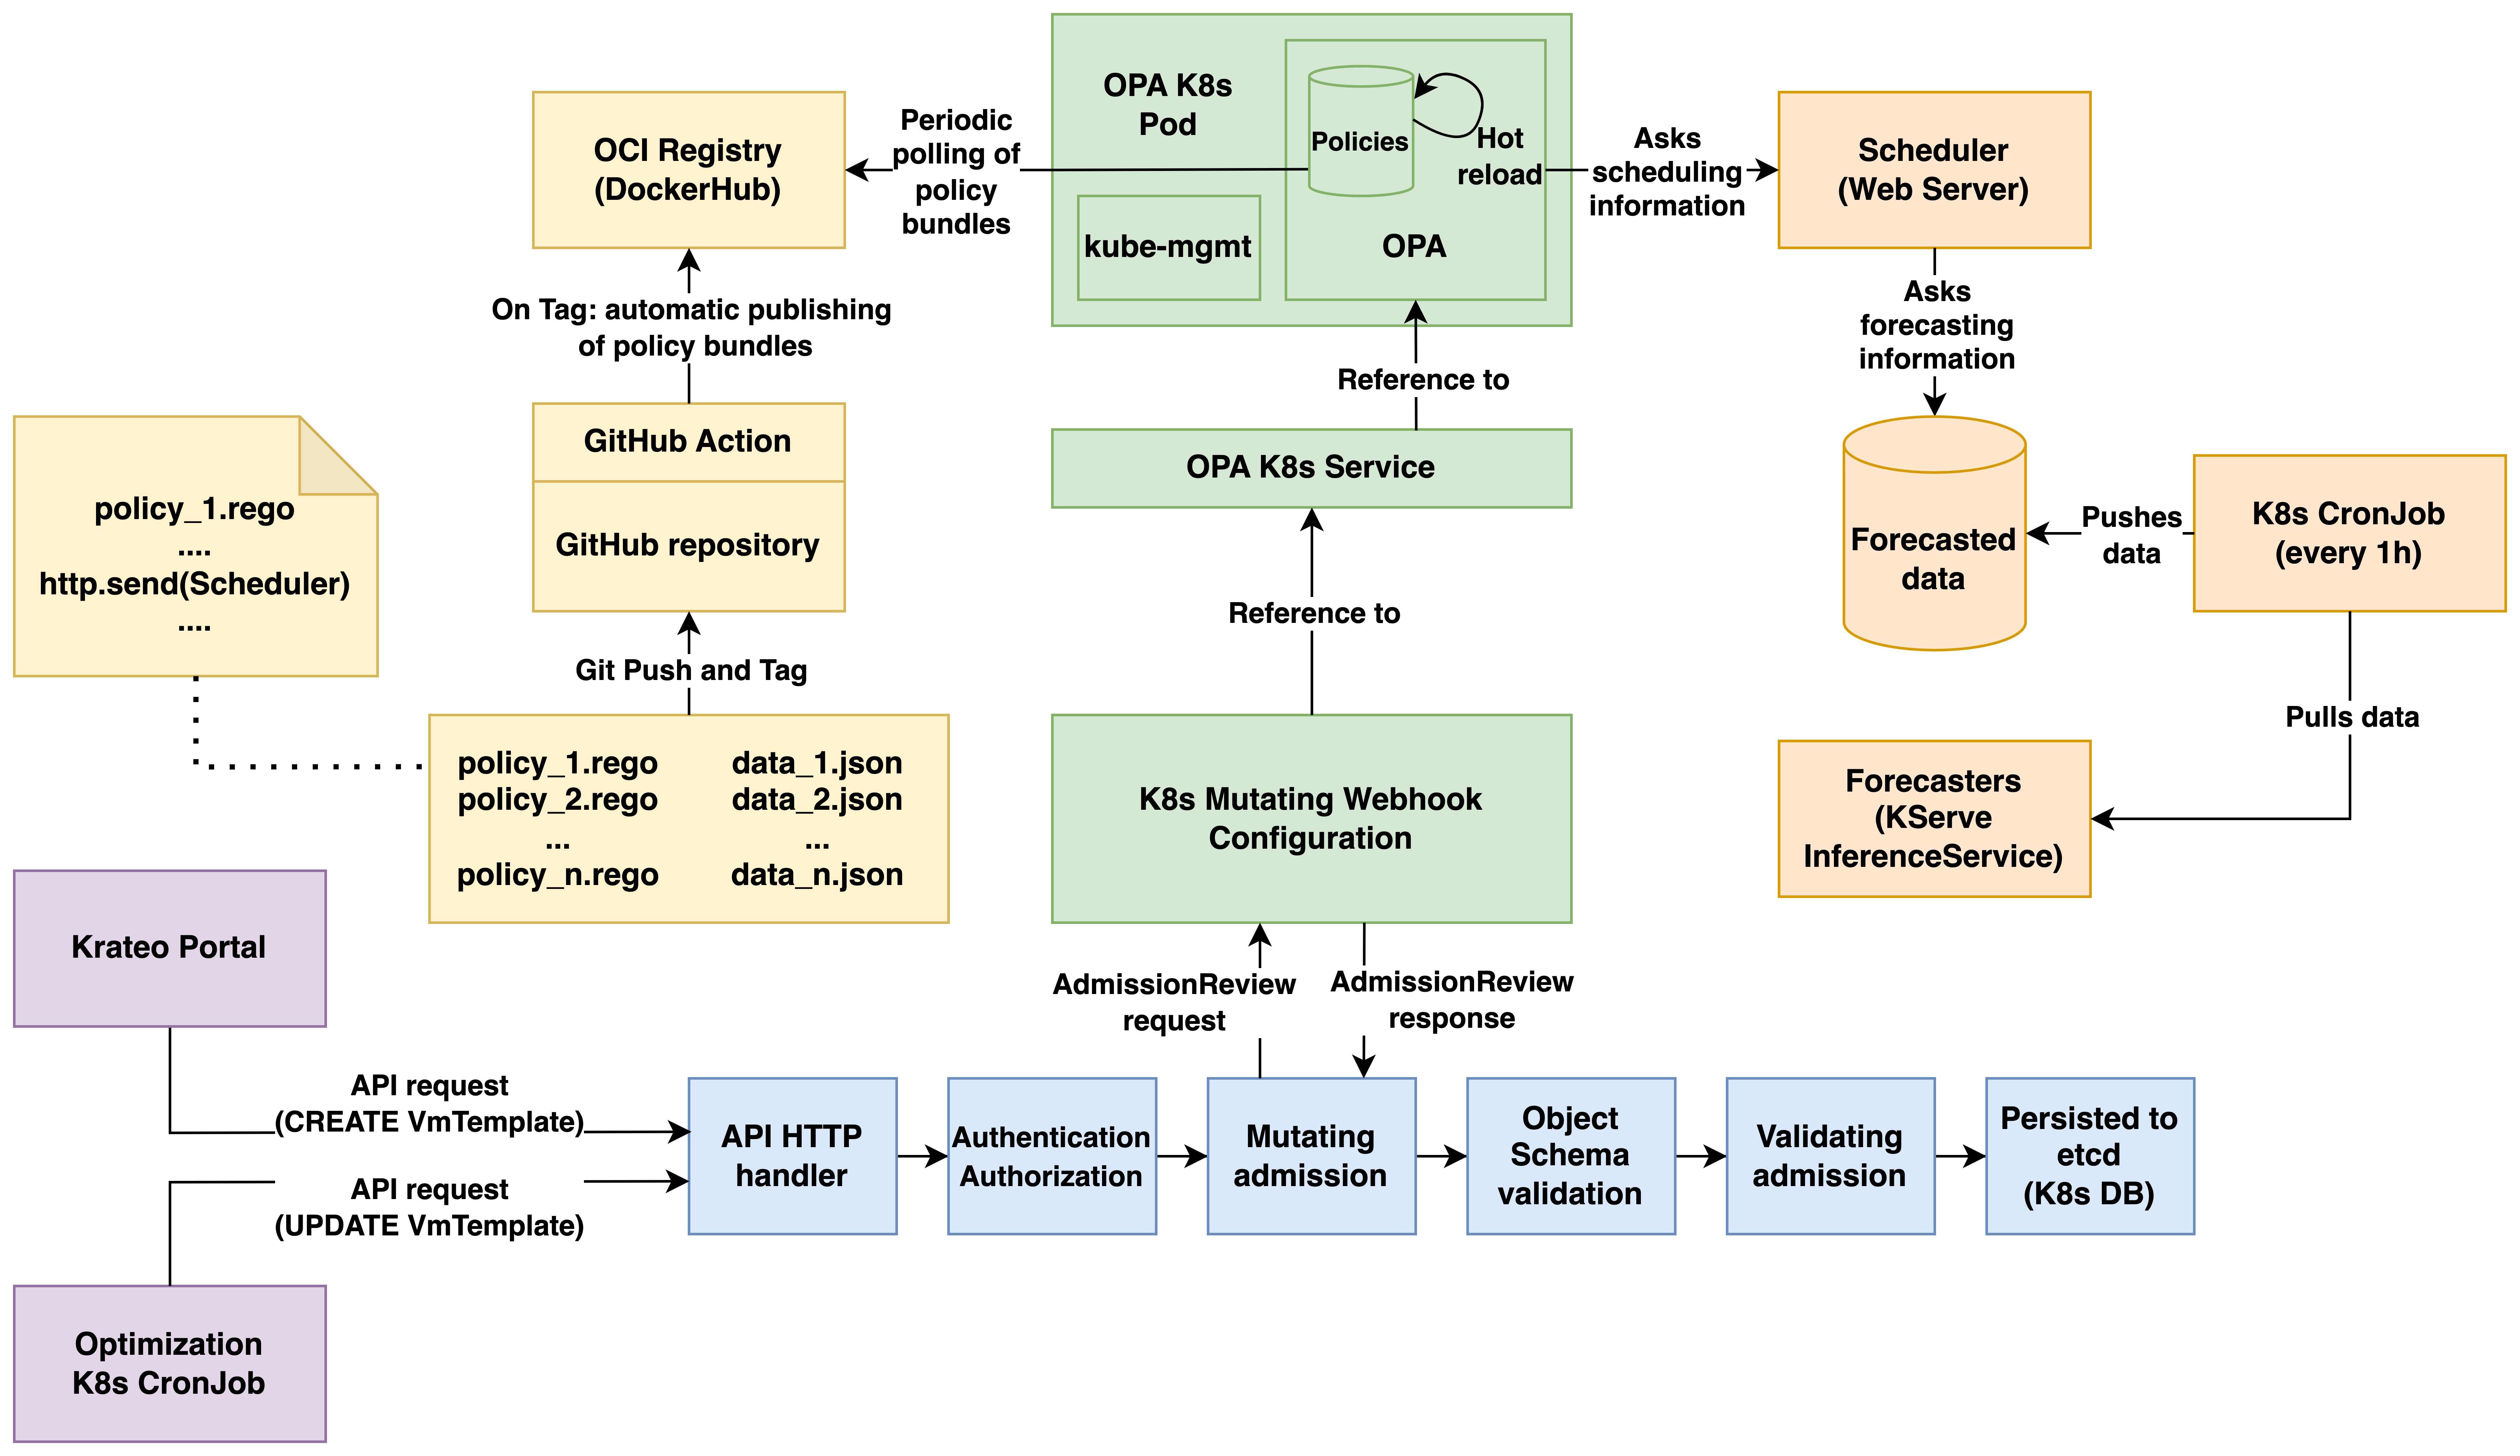
\includegraphics[width=1\linewidth]{images/mutating_webhook+OPA_integration.png}
\caption{Kubernetes mutating webhook + OPA integration}
\label{fig:webhook+opa}
\end{figure}

Figure \ref{fig:webhook+opa} represents the configuration of the Kubernetes Mutating Webhook with the intergeation of Open Policy Agent.
In particular, 




Day 2 operations
The mutating webhook configuration is set on the CREATE and UPDATE operations

UPDATE operation trigger
K8s Cronjob that attach a label to the custom resoruce 

\newpage


\section{MLOps infrastructure}

mlops venn diagram image
to explain what it is

\subsection{MLOps purpose}

MLOps implements DevOps principles, tools and practices into Machine Learning workflows 


purpose: industrialize ML models lifecycle

faster model development

faster model selection and deployment to production

\begin{itemize}[itemsep=0.2pt, topsep=1pt]
  \item[$\bullet$] model tracking (experiments, runs)
  \item[$\bullet$] model selection (model registry)
  \item[$\bullet$] model storage (in buckets)
  \item[$\bullet$] model deployment (inference)
\end{itemize}


allows all the team member to have visibility on the status of the ML models

Instead of having the so-called ``AI Inference Mock Server", treated as a black box returning a scheul;ding time and schedulingLocation

\begin{figure}[htb]
\centering
\includegraphics[width=1\linewidth]{images/mlops_workflow.png}
\caption{MLOps Architecture}
\label{fig:mlops}
\end{figure}


MLFlow framework

KServe framework


\subsection{MLflow}



MLflow Tracking Server


mlflow is compatible with many ML frameworks like sklearn, pythorch


what is a model tracking server
what is a model registry



Mlflow API calls
autolog
infer signature 
important since store 

the end result is a self contained fodler with everythiong needed 
it allows reproducibility 

The training script will also serialise our trained model, leveraging the MLflow Model format.


model/
├── MLmodel
├── model.pkl
├── conda.yaml
└── requirements.tx


additional challenge: CrateDB is not supported natively by mlflow framework
a CrateDB adapter / wrapper is devoloped and mantianed by cratedb community
CrateDB as metadata stoere


SeaweedFS as artifact store
MINio could be an alternative altough it has a restrictive license \cite{minio_license}.



MODEL signature




\subsubsection{Alternative configuration 1}

watchdog
watchdog (pyhton package)
PoC
sidecar container

artifact store not needed

\subsubsection{Alternative configuration 2}

Another possible configuration could be the adoption of just CrateDB as both Metadata Store and Artifact Store.

This would be possible if
CrateDB supports blob storage but not object storage

This solution cannot be implemented yet




\subsection{KServe}


KServe Inference Service


what is
inference server / model server


used to deploy the forecaster (ML model)


uses Istio and Knative under the hood
but a deep descrption of those is out of the scope of this theses.
features: scaling to zero, etc


InferenceService with TorchServe runtime which is the default installed serving runtime for PyTorch models.

Kserve project proposes a standard protocol for inference servers.
The version 2 of the KServe Inference Protocol is the Open Inference Protocol.



\subsubsection{Open Inference Protocol}


\begin{table}[h!]
\centering
\begin{tabular}{|l|l|l|}
\hline
\textbf{API}    & \textbf{Verb} & \textbf{Path}                                                                                         \\ \hline
Inference       & POST          & v2/models/{[}/versions/\textless{}model\_version\textgreater{}{]}/infer                               \\ \hline
Model Ready     & GET           & v2/models/\textless{}model\_name\textgreater{}{[}/versions/{]}/ready                                  \\ \hline
Model Metadata  & GET           & v2/models/\textless{}model\_name\textgreater{}{[}/versions/\textless{}model\_version\textgreater{}{]} \\ \hline
Server Ready    & GET           & v2/health/ready                                                                                       \\ \hline
Server Live     & GET           & v2/health/live                                                                                        \\ \hline
Server Metadata & GET           & v2                                                                                                    \\ \hline
\end{tabular}
\end{table}





adopted by NVIDIA



multi model deployment



our strategy:
1 model per region
1 generic model? as fallback if specific model is not available?




Kserve "stack"

Kserve

in kserve 0.14.1
clusterservingruntimes
supported are 10
among which 
torchserve

clusterservingruntimes -> kserve-mlserver (supported models: sklearn, xgboost, lightgbm, mlflow)

mlserver









serving runtimes

Seldon MLserver


accorgimenti: \\

\lstset{style=python}
\begin{lstlisting}[caption={Wrapping a PyTorch Model}, label={lst:wrapped_model}]
import torch

class WrappedModel(torch.nn.Module):
    def __init__(self, original_model):
        super().__init__()
        self.original_model = original_model

    def forward(self, *args, **kwargs):
        return self.original_model(*args, **kwargs)['prediction_outputs']

# Wrap the existing model
model = WrappedModel(model)

# Now calling model() will return only 'prediction_outputs' (test)
print(model(test_dataset[0]['past_values'].unsqueeze(0)))
\end{lstlisting}









\section{Measurements}
Impact framework (by green software foundation)

\section{End-to-End workflow}
\label{sec:e2eflow}

swim lanes chart figure







Table for recap of all tools used

Kubernetes
- Krateo
Helm
    Helm charts
    Helm templating
    Helm lookup function

- VmTemplate Krateo Composition Definition
- Azure K8s Operator
- GCP K8s Operator
- AWS K8s Operator
- K8s mutating webhook configuration
- OPA server
- opa policies
- OPA bundles
- MLflow tracking server (+ metadata store & artifact store)
- Forecaster (deployed as KServe InferenceService)


\newpage

